% Options for packages loaded elsewhere
\PassOptionsToPackage{unicode}{hyperref}
\PassOptionsToPackage{hyphens}{url}
\documentclass[
]{article}
\usepackage{xcolor}
\usepackage[left=1in,right=1in,top=2in,bottom=1in]{geometry}
\usepackage{amsmath,amssymb}
\setcounter{secnumdepth}{-\maxdimen} % remove section numbering
\usepackage{iftex}
\ifPDFTeX
  \usepackage[T1]{fontenc}
  \usepackage[utf8]{inputenc}
  \usepackage{textcomp} % provide euro and other symbols
\else % if luatex or xetex
  \usepackage{unicode-math} % this also loads fontspec
  \defaultfontfeatures{Scale=MatchLowercase}
  \defaultfontfeatures[\rmfamily]{Ligatures=TeX,Scale=1}
\fi
\usepackage{lmodern}
\ifPDFTeX\else
  % xetex/luatex font selection
\fi
% Use upquote if available, for straight quotes in verbatim environments
\IfFileExists{upquote.sty}{\usepackage{upquote}}{}
\IfFileExists{microtype.sty}{% use microtype if available
  \usepackage[]{microtype}
  \UseMicrotypeSet[protrusion]{basicmath} % disable protrusion for tt fonts
}{}
\makeatletter
\@ifundefined{KOMAClassName}{% if non-KOMA class
  \IfFileExists{parskip.sty}{%
    \usepackage{parskip}
  }{% else
    \setlength{\parindent}{0pt}
    \setlength{\parskip}{6pt plus 2pt minus 1pt}}
}{% if KOMA class
  \KOMAoptions{parskip=half}}
\makeatother
\usepackage{color}
\usepackage{fancyvrb}
\newcommand{\VerbBar}{|}
\newcommand{\VERB}{\Verb[commandchars=\\\{\}]}
\DefineVerbatimEnvironment{Highlighting}{Verbatim}{commandchars=\\\{\}}
% Add ',fontsize=\small' for more characters per line
\usepackage{framed}
\definecolor{shadecolor}{RGB}{248,248,248}
\newenvironment{Shaded}{\begin{snugshade}}{\end{snugshade}}
\newcommand{\AlertTok}[1]{\textcolor[rgb]{0.94,0.16,0.16}{#1}}
\newcommand{\AnnotationTok}[1]{\textcolor[rgb]{0.56,0.35,0.01}{\textbf{\textit{#1}}}}
\newcommand{\AttributeTok}[1]{\textcolor[rgb]{0.13,0.29,0.53}{#1}}
\newcommand{\BaseNTok}[1]{\textcolor[rgb]{0.00,0.00,0.81}{#1}}
\newcommand{\BuiltInTok}[1]{#1}
\newcommand{\CharTok}[1]{\textcolor[rgb]{0.31,0.60,0.02}{#1}}
\newcommand{\CommentTok}[1]{\textcolor[rgb]{0.56,0.35,0.01}{\textit{#1}}}
\newcommand{\CommentVarTok}[1]{\textcolor[rgb]{0.56,0.35,0.01}{\textbf{\textit{#1}}}}
\newcommand{\ConstantTok}[1]{\textcolor[rgb]{0.56,0.35,0.01}{#1}}
\newcommand{\ControlFlowTok}[1]{\textcolor[rgb]{0.13,0.29,0.53}{\textbf{#1}}}
\newcommand{\DataTypeTok}[1]{\textcolor[rgb]{0.13,0.29,0.53}{#1}}
\newcommand{\DecValTok}[1]{\textcolor[rgb]{0.00,0.00,0.81}{#1}}
\newcommand{\DocumentationTok}[1]{\textcolor[rgb]{0.56,0.35,0.01}{\textbf{\textit{#1}}}}
\newcommand{\ErrorTok}[1]{\textcolor[rgb]{0.64,0.00,0.00}{\textbf{#1}}}
\newcommand{\ExtensionTok}[1]{#1}
\newcommand{\FloatTok}[1]{\textcolor[rgb]{0.00,0.00,0.81}{#1}}
\newcommand{\FunctionTok}[1]{\textcolor[rgb]{0.13,0.29,0.53}{\textbf{#1}}}
\newcommand{\ImportTok}[1]{#1}
\newcommand{\InformationTok}[1]{\textcolor[rgb]{0.56,0.35,0.01}{\textbf{\textit{#1}}}}
\newcommand{\KeywordTok}[1]{\textcolor[rgb]{0.13,0.29,0.53}{\textbf{#1}}}
\newcommand{\NormalTok}[1]{#1}
\newcommand{\OperatorTok}[1]{\textcolor[rgb]{0.81,0.36,0.00}{\textbf{#1}}}
\newcommand{\OtherTok}[1]{\textcolor[rgb]{0.56,0.35,0.01}{#1}}
\newcommand{\PreprocessorTok}[1]{\textcolor[rgb]{0.56,0.35,0.01}{\textit{#1}}}
\newcommand{\RegionMarkerTok}[1]{#1}
\newcommand{\SpecialCharTok}[1]{\textcolor[rgb]{0.81,0.36,0.00}{\textbf{#1}}}
\newcommand{\SpecialStringTok}[1]{\textcolor[rgb]{0.31,0.60,0.02}{#1}}
\newcommand{\StringTok}[1]{\textcolor[rgb]{0.31,0.60,0.02}{#1}}
\newcommand{\VariableTok}[1]{\textcolor[rgb]{0.00,0.00,0.00}{#1}}
\newcommand{\VerbatimStringTok}[1]{\textcolor[rgb]{0.31,0.60,0.02}{#1}}
\newcommand{\WarningTok}[1]{\textcolor[rgb]{0.56,0.35,0.01}{\textbf{\textit{#1}}}}
\usepackage{graphicx}
\makeatletter
\newsavebox\pandoc@box
\newcommand*\pandocbounded[1]{% scales image to fit in text height/width
  \sbox\pandoc@box{#1}%
  \Gscale@div\@tempa{\textheight}{\dimexpr\ht\pandoc@box+\dp\pandoc@box\relax}%
  \Gscale@div\@tempb{\linewidth}{\wd\pandoc@box}%
  \ifdim\@tempb\p@<\@tempa\p@\let\@tempa\@tempb\fi% select the smaller of both
  \ifdim\@tempa\p@<\p@\scalebox{\@tempa}{\usebox\pandoc@box}%
  \else\usebox{\pandoc@box}%
  \fi%
}
% Set default figure placement to htbp
\def\fps@figure{htbp}
\makeatother
\setlength{\emergencystretch}{3em} % prevent overfull lines
\providecommand{\tightlist}{%
  \setlength{\itemsep}{0pt}\setlength{\parskip}{0pt}}
\usepackage{tcolorbox}
\tcbuselibrary{listingsutf8}
\usepackage{listings}
\usepackage{xcolor}
\usepackage{chngcntr}
\newcounter{chapter}
\setcounter{chapter}{2}
\counterwithin{table}{chapter}
\usepackage{booktabs}
\usepackage{longtable}
\usepackage{array}
\usepackage{multirow}
\usepackage{wrapfig}
\usepackage{float}
\usepackage{colortbl}
\usepackage{pdflscape}
\usepackage{tabu}
\usepackage{threeparttable}
\usepackage{threeparttablex}
\usepackage[normalem]{ulem}
\usepackage{makecell}
\usepackage{xcolor}
\usepackage{bookmark}
\IfFileExists{xurl.sty}{\usepackage{xurl}}{} % add URL line breaks if available
\urlstyle{same}
\hypersetup{
  pdftitle={Chapter 2: Investigating the Memory of Events Using N-Grams, Controlled Vocabulary, and Joins},
  hidelinks,
  pdfcreator={LaTeX via pandoc}}

\title{Chapter 2: Investigating the Memory of Events Using N-Grams,
Controlled Vocabulary, and Joins}
\author{}
\date{\vspace{-2.5em}}

\begin{document}
\maketitle

Computational methods support inquiry into how the discourses and events
in the past shape current-day political change. It is common in speeches
for political actors to reference the events of the past -- whether
American politicians reference the Tea Party or British parliamentarians
reference the events of the Second World War. Speakers in parliament
also acknowledge contemporary public protests as a source of political
legitimacy. But the number, intensity, and specific events referenced
change over time. What can we learn about how political reforms were
made in the past from reviewing how politicians of the past referenced
events?

In this chapter, we will explore questions such as these: In the lead-up
to the Great Reform Act of 1832, when the middle class got the vote in
Britain, which historical references were on the table? Which members of
parliament contributed the most to the debate about the Abolition of
Slavery in 1833, and of these speakers, whose language reflected the
most on the lived experience of toil and cruelty in the system of
slavery? Which historical and contemporary events were referenced the
most by members of parliament in the era of the Second Reform Act of
1867, when working-class people got the vote for the first time?

This chapter builds upon a sense of how to leverage computational
historical thinking to create insight about history. It introduces
counting n-grams, or multiword phrases. It also introduces the use of a
``controlled vocabulary,'' that is, a historian-curated list of
important words and phrases, to explore which events were spoken about
in parliament during the 1830s.

This chapter builds on the previous to introduce analysts to fundamental
data processing techniques in R, commonly used for preparing data for
analysis. A key task in data analysis is summarizing a dataset's
characteristics to gain insights into the features of the corpus.
Scholars have drawn attention to how th immediacy of computational text
analysis--its perceived automation in transforming a raw, messy corpus
into a curated object of analysis--masks the degree of transformation
that is enacted on the text's ``original'' and intermediary data
structures (Palermo 2017). In this chapter, we draw attention to each
step in data processing, emphasizing how intermediary data wrangling
steps contributes to the creation of new knowledge.

One essential concept in data processing is ``joining'' datasets. A join
combines two datasets into one, allowing us to analyze parliamentary
texts alongside metadata such as speaker information, dates, and
significant events. Additionally, this chapter teaches readers how to
work with event-based data, including years, months, and dates. By
moving through the data processing steps one-by-one, we draw on Paul
Fyfe's framing of ``data mining'' as ``data archaeology,'' shifting
attention away from analysis as a final product and instead
foregrounding the transformational work of data processing as a central
part of the analytical process (Fyfe 2016).

As with the previous chapter, this chapter will emphasize the skills of
moving from analyzing text as data to performing a close reading of
historical speeches in context. It models the iterative process of
working with a controlled vocabulary and reading words in context with
the idea of demonstrating a method of inquiry about how and why events
happen. The approach we model provides analysts with the tools of
deciding for themselves how the patterns identified throughout text
mining relate back to their primary sources, that is, the full Hansard
debates. As we had previously discussed, our analytic process is
iterative, emphasizing that researchers transition from data processing
to counting words to applying metrics on those word counts to
visualizing trends, and then repeating this deductive process.
Throughout the process, it may prove valuable to inspect and re-evaluate
the intermediary steps that were taken to arrive at any conclusions
about the corpus. This cyclical process may lead to additional
historical questions and associations, which may mean more measuring,
more visualization, and more guided reading in pursuit of a historical
analysis.

\subsection{Joining Debate Metadata}\label{joining-debate-metadata}

We have previously seen how to load the text from a single decade of the
Hansard debates. But what should we do if we want to work with not only
the text, but also important information like the name of the speaker
who gave the speech and the date on which the speech was given?

First we can load the text data from the 1860s speeches, recalling that
one of the columns, \texttt{sentence\_id}, refers to the number of each
sentence and its location in the nineteenth-century printed volumes of
Hansard's parliamentary debates, referenced by series (``S''), volume
(``V''), and page (``P''). Sentences are listed in the order in which
they appeared on the page.

\begin{Shaded}
\begin{Highlighting}[]
\CommentTok{\# Use the hansardr library to load the debate text}
\FunctionTok{library}\NormalTok{(hansardr)}

\FunctionTok{data}\NormalTok{(}\StringTok{"hansard\_1860"}\NormalTok{)}
\end{Highlighting}
\end{Shaded}

\begin{Shaded}
\begin{Highlighting}[]
\FunctionTok{kable}\NormalTok{(df\_head, }
      \AttributeTok{format =} \StringTok{"latex"}\NormalTok{, }
      \AttributeTok{booktabs =} \ConstantTok{TRUE}\NormalTok{, }
      \AttributeTok{linesep =} \StringTok{""}\NormalTok{,}
      \AttributeTok{caption =} \StringTok{"Sample sentences from 1860s Hansard, including each sentence\textquotesingle{}s }
\StringTok{                unique identifier and the corresponding text as extracted from the debate transcripts."}\NormalTok{) }\SpecialCharTok{\%\textgreater{}\%}
  \FunctionTok{kable\_styling}\NormalTok{(}\AttributeTok{latex\_options =} \FunctionTok{c}\NormalTok{(}\StringTok{"scale\_down"}\NormalTok{, }\StringTok{"repeat\_header"}\NormalTok{),}
                \AttributeTok{table.envir =} \ConstantTok{FALSE}\NormalTok{) }\SpecialCharTok{\%\textgreater{}\%}
  \FunctionTok{column\_spec}\NormalTok{(}\FunctionTok{which}\NormalTok{(}\FunctionTok{colnames}\NormalTok{(df\_head) }\SpecialCharTok{==} \StringTok{"text"}\NormalTok{), }
              \AttributeTok{latex\_column\_spec =} \StringTok{"p\{12cm\}"}\NormalTok{, }
              \AttributeTok{latex\_valign =} \StringTok{"top"}\NormalTok{)}
\end{Highlighting}
\end{Shaded}

\begin{table}
\centering
\caption{\label{tab:unnamed-chunk-3}Sample sentences from 1860s Hansard, including each sentence's 
                unique identifier and the corresponding text as extracted from the debate transcripts.}
\centering
\resizebox{\ifdim\width>\linewidth\linewidth\else\width\fi}{!}{
\begin{tabular}[t]{lp{12cm}}
\toprule
sentence\_id & text\\
\midrule
S3V0156P0\_0 & which had been prorogued successively to the 27th October, thence to the 15th December, and thence to the 24th January, met this day for Despatch of Business.\\
S3V0156P0\_1 & being seated on the Throne, and the Commons being at the Bar, with their Speaker, HER MAJESTY was pleased to make a most gracious Speech to both Houses of Parliament, as follows:—\\
S3V0156P0\_2 & in rising to move that an humble Address be presented by this House in answer to Her Majesty's most gracious Speech, said:—\\
S3V0156P0\_3 & My Lords, it is with diffidence that I rise to address your Lordships for the first time, and the greater is that diffidence when I recollect that although for many years I had the honour of a seat in the other House of Parliament, I remained throughout that time a silent actor in all the scenes to which my duties called me; but I will be brief, and the observations which I make shall be few, and I trust you will not weigh in too nice a balance any expressions which may fall from me on this occasion.\\
S3V0156P0\_4 & We hear from Her gracious Majesty that it is with gratification\\
\bottomrule
\end{tabular}}
\end{table}

Next, we can load the metadata corresponding with the Hansard debate
text.

\begin{Shaded}
\begin{Highlighting}[]
\FunctionTok{data}\NormalTok{(}\StringTok{"debate\_metadata\_1860"}\NormalTok{)}
\end{Highlighting}
\end{Shaded}

\begin{table}
\centering
\caption{\label{tab:unnamed-chunk-5}Debate-level metadata from 1860s Hansard, including each sentence's identifier, the date of the speech, and the title of the corresponding debate.}
\centering
\resizebox{\ifdim\width>\linewidth\linewidth\else\width\fi}{!}{
\begin{tabular}[t]{lll}
\toprule
sentence\_id & speechdate & debate\\
\midrule
S3V0156P0\_0 & 1860-01-24 & MEETING OF THE PARLIAMENT.\\
S3V0156P0\_1 & 1860-01-24 & THE QUEEN'S SPEECH.\\
S3V0156P0\_2 & 1860-01-24 & ADDRESS IN ANSWER TO HER MAJESTY'S SPEECH.\\
S3V0156P0\_3 & 1860-01-24 & ADDRESS IN ANSWER TO HER MAJESTY'S SPEECH.\\
S3V0156P0\_4 & 1860-01-24 & ADDRESS IN ANSWER TO HER MAJESTY'S SPEECH.\\
\bottomrule
\end{tabular}}
\end{table}

\texttt{hansardr} includes detailed contextual information for each of
the speeches, using the same system of references that we saw in the
previous data set -- series, volume, page, and sentence number. In the
\texttt{debate\_metadata} dataset, however, there is no ``text'' column,
but rather a series of columns that illuminate multiple ``fields'' of
each sentence: the speech date (recorded as ``speechdate'' within the
data) for when the speech was given and the official title of the
``debate'' in which the sentence was spoken.

In addition to the debate metadata, \texttt{hansardr} provides two
additional metadata files: \texttt{speaker\_metadata\_1860} and
\texttt{file\_metadata\_1860}.

\begin{Shaded}
\begin{Highlighting}[]
\CommentTok{\# Load Hansard speaker metadata for 1860 }
\FunctionTok{data}\NormalTok{(}\StringTok{"speaker\_metadata\_1860"}\NormalTok{)}
\end{Highlighting}
\end{Shaded}

\begin{table}
\centering
\caption{\label{tab:unnamed-chunk-7}Speaker-level metadata for sample sentences from the 1860 Hansard corpus, including the recorded speaker name, the algorithmically suggested speaker match, and indicators for name ambiguity, fuzzy matching, and ignored cases.}
\centering
\resizebox{\ifdim\width>\linewidth\linewidth\else\width\fi}{!}{
\begin{tabular}[t]{lllrrr}
\toprule
sentence\_id & speaker & suggested\_speaker & ambiguous & fuzzy\_matched & ignored\\
\midrule
S3V0156P0\_0 & THE PARLIAMENT, &  & 0 & 0 & 0\\
S3V0156P0\_1 & THE QUEEN & peter\_quinn\_4670 & 0 & 1 & 0\\
S3V0156P0\_2 & EARL FITZWILLIAM, & charles\_fitzwilliam\_1441 & 0 & 0 & 0\\
S3V0156P0\_3 & EARL FITZWILLIAM, & charles\_fitzwilliam\_1441 & 0 & 0 & 0\\
S3V0156P0\_4 & EARL FITZWILLIAM, & charles\_fitzwilliam\_1441 & 0 & 0 & 0\\
\bottomrule
\end{tabular}}
\end{table}

The \texttt{speaker\_metadata\_1860} dataset provides information about
the ``speaker'' of each sentence as the MP's name was recorded in the
original Hansard debates. It also includes a ``suggested speaker''
column, which contains a disambiguated version of the speaker names
where ambiguous or inconsistent references to the same individual have
been resolved into a single, standardized name, allowing for more
accurate identification of MPs across the corpus.

The ``suggested speakers'' came from a large-scale disambiguation effort
where the authors of this book disambiguated speaker names, building
upon the work completed by the Digging into Linked Parliamentary Data
Project and the Egger and Spirling database (Eggers and Spirling 2014;
Winters and Steer 2013). Our disambiguation effort was designed to
address these problems: speakers may have been called only by temporary
office titles (like ``Prime Minister''); speakers may have been called
only by their peerage titles (such as ``Duke'' or ``Viscount'');a single
name might have several permutations (such as W. Gladstone, W. E.
Gladstone, or William Gladstone all referring to the same Mr.~William
Ewart Gladstone); speakers may have shared the exact name with someone
else who was active during the same period (like the two different Sir
Robert Peels in the early 19th-century); speaker names may contain OCR
errors; speaker names might have spelling inconsistencies due to how
they were originally recorded during the 19th-century; some speakers
were misrecorded, such as they were called by the wrong title.

By providing both the original speaker field as well as the
disambiguated version, our version of the Hansard dataset preserves the
original historical recording and draws attention to the data
transformation that occurred in the speaker field before the corpus was
packed into \texttt{hansardr}. The purpose of including the ``suggested
speakers'' field is to support computational analysis by linking variant
or ambiguous names to consistent, canonical speaker identities for a
more reliable analysis.

However, we also advise discretion. While disambiguation significantly
improves analysis by standardizing speaker identities, it is not without
limitations. In some cases, speakers may be incorrectly matched or
mislabeled by the algorithm. In others, no suggested speaker name is
provided because the necessary metadata was unavailable, and the sheer
number of speakers made manual correction infeasible within our project
timeline. To address these challenges, we have uploaded the Hansard
corpus to Democracy Viewer, an online text mining and data sharing
platform where researchers can also submit corrections to the corpus
(Buongiorno et al., 2023). Over time, we plan to incorporate data set
improvements into future releases of the \texttt{hansardr} package.

Additionally, disambiguation can obscure the nuances of the original
records, such as shifts in titles or the historical importance of
misspellings for understanding contemporary spelling conventions or
clerical practices. Due to the historical richness of original speaker
names, we provide both the original speaker field and the disambiguated
version, so that researchers can critically assess and, if desired, use
the original speaker name data instead.

Lastly, \texttt{hansardr} provides file metadata. For example, the
\texttt{file\_metadata\_1860} dataset provides metadata about the
records themselves, including the ID for the original source file, and
the column in which the text appears.

\begin{Shaded}
\begin{Highlighting}[]
\CommentTok{\# Load Hansard file metadata for 1860 }
\FunctionTok{data}\NormalTok{(}\StringTok{"file\_metadata\_1860"}\NormalTok{)}
\end{Highlighting}
\end{Shaded}

\begin{table}
\centering
\caption{\label{tab:unnamed-chunk-9}Source-file metadata for selected sentences from the 1860 Hansard corpus, 
    including the identifiers for the sentence, speech, and debate, as well as the source 
    file, source image, and original column location.}
\centering
\resizebox{\ifdim\width>\linewidth\linewidth\else\width\fi}{!}{
\begin{tabular}[t]{lrrllr}
\toprule
sentence\_id & speech\_id & debate\_id & src\_file\_id & src\_image & src\_column\\
\midrule
S3V0156P0\_0 & 258488 & 30416 & S3V0156P0 & S3V0156P0I0033 & 1\\
S3V0156P0\_1 & 258489 & 30417 & S3V0156P0 & S3V0156P0I0033 & 1\\
S3V0156P0\_2 & 258490 & 30418 & S3V0156P0 & S3V0156P0I0036 & 7\\
S3V0156P0\_3 & 258490 & 30418 & S3V0156P0 & S3V0156P0I0036 & 7\\
S3V0156P0\_4 & 258490 & 30418 & S3V0156P0 & S3V0156P0I0036 & 7\\
\bottomrule
\end{tabular}}
\end{table}

We have chosen to store the debate text (\texttt{hansard\_1860})
separately from the contextual information about each speech (for
example, \texttt{debate\_metadata\_1860} or
\texttt{speaker\_metadata\_1860}), as well as the information about each
hard copy file containing the speeches (\texttt{file\_metadata\_1860}).
We subsetted the data into individual files because the data for each
decade is quite large. Processing such a large dataset can exceed a
computer's resources, such as its memory. In other cases, we chose to
exclude certain fields from processing if they were not immediately
relevant to our analysis, as doing so reduces memory usage and improves
overall processing speed so that we can focus on our research instead of
waiting too long for any intermediary processing step to complete.
Furthermore, many operations in this book -- for instance, counting
words per decade -- require just a few datasets loaded at a time.

Many kinds of analyses will require working with multiple datasets from
\texttt{hansardr} joined together. We will use the function
\texttt{left\_join()} to join the annotated information about speech
context with each of the speech text. A left join returns every record
from the data frame specified by the left-most argument, and all the
matched records from the data frame on the right.

\begin{Shaded}
\begin{Highlighting}[]
\CommentTok{\# Load the tidyverse}
\FunctionTok{library}\NormalTok{(}\StringTok{"tidyverse"}\NormalTok{)}

\CommentTok{\# Join the Hansard debate text with the debate metadata into a single data frame}
\CommentTok{\# left\_join() will automatically detect that both datasets share the sentence\_id }
\NormalTok{hansard\_1860 }\OtherTok{\textless{}{-}} \FunctionTok{left\_join}\NormalTok{(hansard\_1860, debate\_metadata\_1860)}

\CommentTok{\# Show the first few rows of the 1860 Hansard debate text}
\NormalTok{hansard\_1860 }\SpecialCharTok{\%\textgreater{}\%}
  \FunctionTok{head}\NormalTok{() }\SpecialCharTok{\%\textgreater{}\%}
  \FunctionTok{mutate}\NormalTok{(}\AttributeTok{text =} \FunctionTok{str\_trunc}\NormalTok{(text, }\DecValTok{120}\NormalTok{)) }\SpecialCharTok{\%\textgreater{}\%}  
  \FunctionTok{kable}\NormalTok{(}\AttributeTok{format =} \StringTok{"latex"}\NormalTok{, }
        \AttributeTok{booktabs =} \ConstantTok{TRUE}\NormalTok{, }
        \AttributeTok{caption =} \StringTok{"Text excerpts from the 1860 Hansard corpus alongside their associated }
\StringTok{                  metadata, including the sentence identifier, speech date, and }
\StringTok{                  debate title."}\NormalTok{) }\SpecialCharTok{\%\textgreater{}\%}
  \FunctionTok{kable\_styling}\NormalTok{(}\AttributeTok{full\_width =} \ConstantTok{FALSE}\NormalTok{, }\AttributeTok{position =} \StringTok{"left"}\NormalTok{) }\SpecialCharTok{\%\textgreater{}\%}
  \FunctionTok{column\_spec}\NormalTok{(}\DecValTok{2}\NormalTok{, }\AttributeTok{width =} \StringTok{"6cm"}\NormalTok{) }\SpecialCharTok{\%\textgreater{}\%}
  \FunctionTok{column\_spec}\NormalTok{(}\DecValTok{4}\NormalTok{, }\AttributeTok{width =} \StringTok{"4cm"}\NormalTok{)}
\end{Highlighting}
\end{Shaded}

\begin{table}

\caption{\label{tab:unnamed-chunk-10}Text excerpts from the 1860 Hansard corpus alongside their associated 
                  metadata, including the sentence identifier, speech date, and 
                  debate title.}
\begin{tabular}[t]{l>{\raggedright\arraybackslash}p{6cm}l>{\raggedright\arraybackslash}p{4cm}}
\toprule
sentence\_id & text & speechdate & debate\\
\midrule
S3V0156P0\_0 & which had been prorogued successively to the 27th October, thence to the 15th December, and thence to the 24th Januar... & 1860-01-24 & MEETING OF THE PARLIAMENT.\\
S3V0156P0\_1 & being seated on the Throne, and the Commons being at the Bar, with their Speaker, HER MAJESTY was pleased to make a m... & 1860-01-24 & THE QUEEN'S SPEECH.\\
S3V0156P0\_2 & in rising to move that an humble Address be presented by this House in answer to Her Majesty's most gracious Speech, ... & 1860-01-24 & ADDRESS IN ANSWER TO HER MAJESTY'S SPEECH.\\
S3V0156P0\_3 & My Lords, it is with diffidence that I rise to address your Lordships for the first time, and the greater is that dif... & 1860-01-24 & ADDRESS IN ANSWER TO HER MAJESTY'S SPEECH.\\
S3V0156P0\_4 & We hear from Her gracious Majesty that it is with gratification & 1860-01-24 & ADDRESS IN ANSWER TO HER MAJESTY'S SPEECH.\\
\addlinespace
S3V0156P0\_5 & She meets her Parliament, that She continues on terms of friendship with all foreign countries; but while there is th... & 1860-01-24 & ADDRESS IN ANSWER TO HER MAJESTY'S SPEECH.\\
\bottomrule
\end{tabular}
\end{table}

Notice that the resulting dataset, \texttt{hansard\_corpus\_1860}, has
information about speaker and date for each sentence of text.

Joins are a crucial concept for combining and analyzing data that is
distributed across multiple datasets. They allow us to link related
information from different tables based on a shared key or common field
thus enabling us to perform analyses of the records in relation to its
metadata.

In the example above, both \texttt{hansard\_1860} and
\texttt{debate\_metadata\_1860} share a column called
\texttt{sentence\_id}. The shared \texttt{sentence\_id} column acts as a
common identifier, enabling us to link the speaker and date information
from one dataset to the corresponding text of the speech in the other
dataset. By using this common identifier, the two datasets can be
``joined'' together to create a single, unified dataset that we will use
for text processing.

Thus joins are so important because it is through linking the records to
their metadata that we are able to break text into subsets and analyze
change over time, or create a biography of any individual speaker. We
can explore the words invoked in parliament in the months leading up to
August 15, 1867, when most working-class men in Britain finally achieved
the right to vote.

\subsection{Multiword Phrases}\label{multiword-phrases}

Beyond analyzing individual words, an analyst may want to explore
multiword phrases. Multiword phrases contain formulations of concepts
that had powerful political, social, and cultural meaning to speakers,
for example, ``the will of the people,'' a phrase that has been invoked
by both radicals and conservatives to support extremely different
imaginations of the people. That is, speakers who invoked ``the will of
the people'' might have been bolstering the importance of their speech
by gesturing towards their status as a representative of the workers
whose labor is the source of all political legitimacy. On the other
hand, some speakers might have used the same phrase -- ``the will of the
people'' -- to kindle an imagination of parliament as a zone a
traditional folk whose national identity legitimizes a politics of
excluding from citizenship or rights people with certain racial or
immigration status. The question becomes: which version of the people
was being represented in the discourse in question?

The analyst cannot anticipate in advance how such a phrase might have
been used. The only way of gaining knowledge from a count of phrases is
to ``validate'' one theory or the other by gaining more information.

We could, in theory, contrive computational approaches to help us
discern why people invoked ``the will of the people.'' But in \emph{Text
Mining for Historical Analysis}, we often want to move from identifying
a data-driven phenomenon to gaining more information about historical
context by reading the actual speeches. Our approach modeled
approach--moving from a visualization overview back to the data
itself--provides insight into the rich nuances suggested by speakers by
giving us perspective into how they invoke particular phrase in the
original records. While visualizations might demonstrate that a
parliamentarian invoked a phrase, they may not clearly demonstrate how
that phrase was invoked.

Accordingly, in the sections below, we will begin by counting phrases,
but that is not where we will end. We will return to the original
speeches to read more deeply.

\subsubsection{Finding Bigrams}\label{finding-bigrams}

While there are several approaches to finding multiword phrases, we will
demonstrate finding them by tokenizing the text into bigrams.

The following code filters the speeches of the 1860s for the first
months of 1867 before the vote on the Second Reform Act, which gave
Britain's urban working-class men the right to vote. We also introduce a
new package, \texttt{lubridate}, which can be installed in the usual way
using \texttt{install.packages()}.

\begin{Shaded}
\begin{Highlighting}[]
\CommentTok{\# load packages for tokenization and date handling}
\FunctionTok{library}\NormalTok{(}\StringTok{"tidytext"}\NormalTok{)   }
\end{Highlighting}
\end{Shaded}

\begin{verbatim}
## Warning: package 'tidytext' was built under R version 4.5.2
\end{verbatim}

\begin{Shaded}
\begin{Highlighting}[]
\FunctionTok{library}\NormalTok{(}\StringTok{"lubridate"}\NormalTok{)  }

\CommentTok{\# create a new data frame "hansard\_1867" from "hansard\_1860" that contains}
\CommentTok{\# data for 1867 }
\NormalTok{hansard\_1867 }\OtherTok{\textless{}{-}}\NormalTok{ hansard\_1860 }\SpecialCharTok{\%\textgreater{}\%} \CommentTok{\# create a new data frame}
  \FunctionTok{mutate}\NormalTok{(}\AttributeTok{year =} \FunctionTok{year}\NormalTok{(speechdate)) }\SpecialCharTok{\%\textgreater{}\%} \CommentTok{\# extract year from speechdate}
  \FunctionTok{filter}\NormalTok{(year }\SpecialCharTok{==} \DecValTok{1867}\NormalTok{, }\CommentTok{\# keep only year 1867}
\NormalTok{         speechdate }\SpecialCharTok{\textless{}=} \FunctionTok{ymd}\NormalTok{(}\StringTok{"1867{-}08{-}15"}\NormalTok{)) }\CommentTok{\# and speechdate before or on august 15}
\end{Highlighting}
\end{Shaded}

Now that we have filtered the dataset for our desired timeline, we can
tokenize the text into bigrams. The order in which we perform data
processing is important. Tokenizing after filtering ensures that we are
working with a smaller and more focused dataset. Working with a smaller
dataset ensures we do not exhaust our computer's resources or its
processing capabilities. Skills for handling a large dataset on a
smaller computer, like a laptop, is paramount to being able to answer
questions while processing large corpora for historical analysis, as we
describe in more detail in subsequent chapters.

The order of our steps is not arbitrary, but the outcome of a deliberate
decision. We could have reversed them---for example, tokenizing the text
before filtering by date. However, that approach would have used more of
our computer's resources, as it would require processing a larger volume
of irrelevant text before narrowing the records down to just the data
needed for our inquiry into a given time period. With large datasets
like Hansard, the sequence of processing steps can significantly impact
whether the data remains manageable.

In turn, the limitations of any computing environment directly shape the
types of analyses we prioritize. In other words, it is not only
theoretical or interpretive concerns that determine our methodological
choices, but also what is computationally feasible. Technical
constraints become analytical constraints.

When working with large-scale historical data, researchers often adapt
their questions, models, and scope to align with the practical
boundaries of a computer's available memory, processing speed, and
storage. Computational limitations might encourage researchers to think
critically and strategically about what kinds of knowledge are worth
pursuing, and how best to pursue them with the tools at hand.

Throughout \emph{Text Mining for Historical Analysis} we have attempted
to limit barriers to processing a dataset as large as Hansard through
our data organization scheme that breaks each decade of text and related
metadata files into their own files, and presents readers with an order
of intermediary data processing that is more efficient for working with
historical data in R.

The following code uses the \texttt{unnest\_tokens()} function, which we
previously used to split text into individual words. This time, we
adjust the function to extract pairs of consecutive words instead. To
focus on pairs of consecutive words instead, we set the token argument
to n-grams, instructing R to create sequences of consecutive words, and
the \texttt{n} argument to \texttt{2}, specifying that each sequence
should consist of two words. The two arguments work together to extract
bigrams.

\begin{Shaded}
\begin{Highlighting}[]
\CommentTok{\# Generate bigrams (two{-}word sequences) from the "text" column of the hansard\_1867 data}
\NormalTok{bigrams\_1867 }\OtherTok{\textless{}{-}}\NormalTok{ hansard\_1867 }\SpecialCharTok{\%\textgreater{}\%} \CommentTok{\# create a new dataset}
  \FunctionTok{unnest\_tokens}\NormalTok{(bigram, text, }\AttributeTok{token =} \StringTok{"ngrams"}\NormalTok{, }\AttributeTok{n =} \DecValTok{2}\NormalTok{) }\CommentTok{\# unnest bigrams }
\end{Highlighting}
\end{Shaded}

\begin{table}
\centering
\caption{\label{tab:unnamed-chunk-13}Raw bigrams extracted from the 1867 Hansard proceedings alongside their associated metadata.}
\centering
\resizebox{\ifdim\width>\linewidth\linewidth\else\width\fi}{!}{
\begin{tabular}[t]{lllrl}
\toprule
sentence\_id & speechdate & debate & year & bigram\\
\midrule
S3V0185P0\_0 & 1867-02-05 & THE QUEEN'S SPEECH. & 1867 & being seated\\
S3V0185P0\_0 & 1867-02-05 & THE QUEEN'S SPEECH. & 1867 & seated on\\
S3V0185P0\_0 & 1867-02-05 & THE QUEEN'S SPEECH. & 1867 & on the\\
S3V0185P0\_0 & 1867-02-05 & THE QUEEN'S SPEECH. & 1867 & the throne\\
S3V0185P0\_0 & 1867-02-05 & THE QUEEN'S SPEECH. & 1867 & throne adorned\\
\bottomrule
\end{tabular}}
\end{table}

Note that the bigrams extracted overlap, as if the same sentence had
been subdivided several times. The presentation of the bigrams is
expected, as bigrams are created by looking at each pair of words in
order, one step at a time---so each new bigram shares a word with the
one before it.

\subsubsection{Counting Bigrams}\label{counting-bigrams}

Now we can count the top bigrams and remove any that contain stop words.
We remove stop words to focus on word pairs that might be more
meaningful for our analysis.

\begin{Shaded}
\begin{Highlighting}[]
\CommentTok{\# remove bigrams that contain any stop words}
\CommentTok{\# keep only bigrams made up of two lowercase alphabetic words}
\NormalTok{clean\_bigrams\_1867 }\OtherTok{\textless{}{-}}\NormalTok{ bigrams\_1867 }\SpecialCharTok{\%\textgreater{}\%}
  \FunctionTok{filter}\NormalTok{(}\SpecialCharTok{!}\FunctionTok{str\_detect}\NormalTok{(bigram, }
                     \FunctionTok{paste0}\NormalTok{(}\StringTok{"}\SpecialCharTok{\textbackslash{}\textbackslash{}}\StringTok{b("}\NormalTok{, }\FunctionTok{paste}\NormalTok{(stop\_words}\SpecialCharTok{$}\NormalTok{word, }\AttributeTok{collapse =} \StringTok{"|"}\NormalTok{), }\StringTok{")}\SpecialCharTok{\textbackslash{}\textbackslash{}}\StringTok{b"}\NormalTok{))) }\SpecialCharTok{\%\textgreater{}\%}
  \FunctionTok{filter}\NormalTok{(}\FunctionTok{str\_detect}\NormalTok{(bigram, }\StringTok{"\^{}[a{-}z]+ [a{-}z]+$"}\NormalTok{))}
\end{Highlighting}
\end{Shaded}

\begin{table}
\centering
\caption{\label{tab:unnamed-chunk-15}Cleaned bigrams from the 1867 Hansard corpus together with their metadata. The cleaned bigrams reflect preprocessing steps that remove stopwords.}
\centering
\resizebox{\ifdim\width>\linewidth\linewidth\else\width\fi}{!}{
\begin{tabular}[t]{lllrl}
\toprule
sentence\_id & speechdate & debate & year & bigram\\
\midrule
S3V0185P0\_0 & 1867-02-05 & THE QUEEN'S SPEECH. & 1867 & throne adorned\\
S3V0185P0\_0 & 1867-02-05 & THE QUEEN'S SPEECH. & 1867 & regal ornaments\\
S3V0185P0\_1 & 1867-02-05 & THE QUEEN'S SPEECH. & 1867 & robes sitting\\
S3V0185P0\_2 & 1867-02-05 & THE QUEEN'S SPEECH. & 1867 & robes commanded\\
S3V0185P0\_2 & 1867-02-05 & THE QUEEN'S SPEECH. & 1867 & gentleman usher\\
\bottomrule
\end{tabular}}
\end{table}

The above code processes the dataset by applying the following
transformations and filters:

\texttt{filter(!str\_detect(...))} - Removes rows where the
\texttt{bigram} column contains any stop word. - It constructs a regular
expression from a list of stop words (\texttt{stop\_words\$word}) by: -
Combining them with the OR operator (\texttt{\textbar{}}). - Surrounding
them with word boundaries (\texttt{\textbackslash{}\textbackslash{}b})
to match complete words only. - Only bigrams without stop words are
retained.

\texttt{filter(str\_detect(bigram,\ "\^{}{[}a-z{]}+\ {[}a-z{]}+\$"))} -
Keeps rows where the \texttt{bigram} column matches a specific pattern:
- The \texttt{bigram} must consist of exactly two lowercase alphabetic
words separated by a single space. - Rows where the \texttt{bigram}
contains numbers, punctuation, or non-lowercase letters are excluded.

We can now count the resulting bigrams.

\begin{Shaded}
\begin{Highlighting}[]
\CommentTok{\# count the frequency of each bigram in the cleaned dataset}
\CommentTok{\# keep the top 100 most frequent bigrams and sort them in descending order}
\NormalTok{top\_bigrams\_1867 }\OtherTok{\textless{}{-}}\NormalTok{ clean\_bigrams\_1867 }\SpecialCharTok{\%\textgreater{}\%}
  \FunctionTok{count}\NormalTok{(bigram) }\SpecialCharTok{\%\textgreater{}\%} \CommentTok{\# count frequency of each bigram}
  \FunctionTok{top\_n}\NormalTok{(}\DecValTok{100}\NormalTok{) }\SpecialCharTok{\%\textgreater{}\%} \CommentTok{\# select top 100 bigrams}
  \FunctionTok{arrange}\NormalTok{(}\FunctionTok{desc}\NormalTok{(n)) }\CommentTok{\# sort bigrams by frequency, highest first}
\end{Highlighting}
\end{Shaded}

\begin{table}
\centering
\caption{\label{tab:unnamed-chunk-17}The most frequent bigrams in the 1867 Hansard corpus, ranked 
    by their number of occurrences.}
\centering
\resizebox{\ifdim\width>\linewidth\linewidth\else\width\fi}{!}{
\begin{tabular}[t]{lr}
\toprule
bigram & n\\
\midrule
noble lord & 1807\\
noble earl & 1538\\
noble friend & 1027\\
roman catholic & 943\\
reform bill & 742\\
\bottomrule
\end{tabular}}
\end{table}

In our list, we see several contemporary rhetorical figures that stem
from the practice of referring to other speakers in parliament as ``my
noble friend'' or ``my learned friend.'' We also see allusions to the
debates over representation and the question of who would have the vote,
especially in the phrases ``household suffrage,'' referencing historical
argument for granting middle-class men the right to vote with the Reform
Bill of 1832, and ``roman catholic,'' a reference to the fact that Roman
Catholics could already vote until the Reform Act of 1834. Only in 1867
did those working-class men get the vote in Britain, and these earlier
precedents were frequently alluded to as a justification.

We also see a reference to ``public meetings.'' Why did speakers in
parliament invoke public meetings in the lead-up to the Second Reform
Act? We will answer this question by reading the original text.

\begin{Shaded}
\begin{Highlighting}[]
\CommentTok{\# Filter the 1867 Hansard speeches to keep only those that mention "public meetings"}
\NormalTok{my\_reading }\OtherTok{\textless{}{-}}\NormalTok{ hansard\_1867 }\SpecialCharTok{\%\textgreater{}\%} \CommentTok{\# create a new dataset}
  \FunctionTok{filter}\NormalTok{(}\FunctionTok{str\_detect}\NormalTok{(text, }\StringTok{"public meetings"}\NormalTok{)) }\CommentTok{\# detect the phrase}

\NormalTok{my\_reading }\SpecialCharTok{\%\textgreater{}\%}
  \FunctionTok{head}\NormalTok{() }\SpecialCharTok{\%\textgreater{}\%}
  \FunctionTok{mutate}\NormalTok{(}\AttributeTok{text =} \FunctionTok{str\_wrap}\NormalTok{(text, }\DecValTok{80}\NormalTok{)) }\SpecialCharTok{\%\textgreater{}\%}
  \FunctionTok{select}\NormalTok{(text) }\SpecialCharTok{\%\textgreater{}\%}
  \FunctionTok{kable}\NormalTok{(}\AttributeTok{format =} \StringTok{"latex"}\NormalTok{, }
        \AttributeTok{booktabs =} \ConstantTok{TRUE}\NormalTok{, }
        \AttributeTok{longtable =} \ConstantTok{TRUE}\NormalTok{, }
        \AttributeTok{escape =} \ConstantTok{FALSE}\NormalTok{,}
        \AttributeTok{caption =} \StringTok{"Sample Hansard text from 1867 containing multiple occurrences }
\StringTok{        of the phrase “public meetings.”"}\NormalTok{) }\SpecialCharTok{\%\textgreater{}\%}
  \FunctionTok{column\_spec}\NormalTok{(}\DecValTok{1}\NormalTok{, }\AttributeTok{width =} \StringTok{"14cm"}\NormalTok{)}
\end{Highlighting}
\end{Shaded}

\begin{longtable}[t]{>{\raggedright\arraybackslash}p{14cm}}
\caption{\label{tab:unnamed-chunk-18}Sample Hansard text from 1867 containing multiple occurrences 
        of the phrase “public meetings.”}\\
\toprule
text\\
\midrule
I am aware that many of the public meetings have declared in favour of manhood
suffrage, but hardly any one in either House of Parliament wishes for such a
suffrage, and if you give the working classes of this country a fair proportion
of votes you may hope to settle this question for a considerable time.\\
They are often drawn up with considerable ability; but they bear the mark, I
think, of a single hand, and though they profess to emanate from public meetings
in the different counties of Nova Scotia, they are—\\
Speeches at public meetings, and the discussions of the press, great as their
influence undoubtedly is, have yet less effect upon public opinion than the
debates of Parliament.\\
I know I shall be asked, from what I have seen in the press, and what has
been said at public meetings, in respect to a plan that has been spoken of for
workhouse and infirmary alteration, ""Why do you not have six or seven large
hospitals, each containing 1, 000 inmates, and conducted upon the principle of
hospitals pure and simple?""\\
Have you not heard or read what has been said at public meetings of every kind?\\
\addlinespace
There have been more than 1, 000 public meetings; at every one, the doors
were open, and any man could come in, whatever his opinions, and the all but
unanimous vote of these meetings has been in favour of something much larger and
more complete than the plan of the right hon.\\
\bottomrule
\end{longtable}

A cursory reading of the sentences suggests that members of parliament
were well aware of massive public meetings where more than a thousand
members of the public showed up support the vote for working-class
people. We read of demonstrations around British Empire, even in Nova
Scotia. We read of members of parliament challenging each other to meet
the demands of the public: ``Have you not heard or read what has been
said?'' We have only skimmed a few sentences, but the material in these
126 rows gives us what we need to understand how members of parliament
talked about public protests in these crucial months of 1867.

Bigrams, however, have limitations. A bigram only looks at one preceding
word, but meaning often depends on words far apart in a sentence.
Observing longer utterances---such as by moving beyond bigrams to
multiword phrases---allows us to capture linguistic meaning that depends
on more distant context than just the immediately preceding word.

\subsubsection{Counting Multiword
Phrases}\label{counting-multiword-phrases}

Text mining also allows us to look for multiword phrases beyond bigrams.
We can look at 5-word phrases from the year 1867. We can also add a line
to filter the n-grams for the presence of the word ``people,'' looking
for voices that refer to democracy, for instance, ``the will of the
people,'' an important concept in the years leading up to 1867, when
working-class men in cities got the right to vote for the first time.
The results will allow us to ask the question: What are the most
frequently-invoked phrases involving ``the people''?

We can use a slight adjustment of the code we used above to count
bigrams to find n-grams of any length. Here is code for finding common
five-word-phrases, filtering them, counting them, and finding the top 50
examples:

\begin{Shaded}
\begin{Highlighting}[]
\CommentTok{\# create 5{-}grams (sequences of 5 consecutive words) from the "text" column}
\CommentTok{\# store the results in a new column called "ngram"}
\CommentTok{\# unnest\_tokens() is used with token = "ngrams" and n = 5 to generate 5{-}word sequences}
\NormalTok{fivegrams\_1867 }\OtherTok{\textless{}{-}}\NormalTok{ hansard\_1867 }\SpecialCharTok{\%\textgreater{}\%} \CommentTok{\# create a new dataset}
  \FunctionTok{unnest\_tokens}\NormalTok{(ngram, text, }\AttributeTok{token =} \StringTok{"ngrams"}\NormalTok{, }\AttributeTok{n =} \DecValTok{5}\NormalTok{) }\CommentTok{\# generate 5{-}grams from text}

\CommentTok{\# filter for 5{-}grams that contain the word "people"}
\CommentTok{\# count the frequency of those 5{-}grams and keep the top 50}
\NormalTok{people\_n\_grams }\OtherTok{\textless{}{-}}\NormalTok{ fivegrams\_1867 }\SpecialCharTok{\%\textgreater{}\%} \CommentTok{\# create a new dataset}
  \FunctionTok{filter}\NormalTok{(}\FunctionTok{str\_detect}\NormalTok{(ngram, }\StringTok{"people"}\NormalTok{)) }\SpecialCharTok{\%\textgreater{}\%} \CommentTok{\# keep 5{-}grams containing "people"}
  \FunctionTok{count}\NormalTok{(ngram) }\SpecialCharTok{\%\textgreater{}\%} \CommentTok{\# count frequency of each 5{-}gram}
  \FunctionTok{top\_n}\NormalTok{(}\DecValTok{50}\NormalTok{) }\CommentTok{\# keep top 50 by count}

\FunctionTok{head}\NormalTok{(people\_n\_grams)}
\end{Highlighting}
\end{Shaded}

\begin{verbatim}
##                          ngram  n
## 1    feelings of the people of  8
## 2     great body of the people 32
## 3 great majority of the people 13
## 4     great mass of the people 15
## 5 majority of the irish people 10
## 6    majority of the people of 27
\end{verbatim}

We see a great many political concepts invoked about what members of
parliament believed they were working for -- the people of Ireland,
England, or the metropolis, their representation, condition, education,
minds, interests, feelings, rights, and welfare. An entire vocabulary of
social engagement and political will was being spelled out.

Reading further down the list of multi-word phrases might give us more
hints about the language with which speakers urged the principle of
representation. Again, the careful analyst would trace the vocabulary
words back to their original context, using the original text of the
speeches to develop an argument about why a phrase like ``the minds of
the people'' was used.

\begin{Shaded}
\begin{Highlighting}[]
\CommentTok{\# Filter the 1867 Hansard speeches to include only rows where the exact phrase }
\CommentTok{\# "minds of the people" appears in the "text" column}
\NormalTok{minds }\OtherTok{\textless{}{-}}\NormalTok{ hansard\_1867 }\SpecialCharTok{\%\textgreater{}\%} \CommentTok{\# create a new dataset}
  \FunctionTok{filter}\NormalTok{(}\FunctionTok{str\_detect}\NormalTok{(text, }\StringTok{"minds of the people"}\NormalTok{)) }\CommentTok{\# detect the phrase}

\NormalTok{minds }\SpecialCharTok{\%\textgreater{}\%}
  \FunctionTok{head}\NormalTok{() }\SpecialCharTok{\%\textgreater{}\%}
  \FunctionTok{mutate}\NormalTok{(}\AttributeTok{text =} \FunctionTok{str\_wrap}\NormalTok{(text, }\DecValTok{80}\NormalTok{)) }\SpecialCharTok{\%\textgreater{}\%}
  \FunctionTok{select}\NormalTok{(text) }\SpecialCharTok{\%\textgreater{}\%}
  \FunctionTok{kable}\NormalTok{(}\AttributeTok{format =} \StringTok{"latex"}\NormalTok{, }
        \AttributeTok{booktabs =} \ConstantTok{TRUE}\NormalTok{, }
        \AttributeTok{longtable =} \ConstantTok{TRUE}\NormalTok{, }
        \AttributeTok{escape =} \ConstantTok{FALSE}\NormalTok{,}
        \AttributeTok{caption =} \StringTok{"Sample Hansard text from 1867 containing multiple }
\StringTok{        occurrences of the phrase “minds of the people.”"}\NormalTok{) }\SpecialCharTok{\%\textgreater{}\%}
  \FunctionTok{column\_spec}\NormalTok{(}\DecValTok{1}\NormalTok{, }\AttributeTok{width =} \StringTok{"14cm"}\NormalTok{)}
\end{Highlighting}
\end{Shaded}

\begin{longtable}[t]{>{\raggedright\arraybackslash}p{14cm}}
\caption{\label{tab:unnamed-chunk-20}Sample Hansard text from 1867 containing multiple 
        occurrences of the phrase “minds of the people.”}\\
\toprule
text\\
\midrule
It is satisfactory to learn that these measures afforded great relief to the
minds of the people of Killarney, and that no further outbreak has occurred,
except, as we understand, that the police barrack at Kells, eight miles from
Cahirciveen, was attacked by the same party which visited Cahirciveen.\\
Its debates have been the principal means by which political wisdom, and the
results arrived at by the patient researches of philosophical inquirers, have
been made gradually to sink into the minds of the people, and truths at first
recognised only by a few of the ablest men of their day, have at length been
practically adopted in legislation.\\
Its debates command nothing like the same interest and attention, and exercise
far less influence for good on the minds of the people.\\
Gentleman the Question of which he had given notice, and was sure the Government
would sacrifice nothing of its importance or dignity by acceding to that
request; and if they could dispense with long debates on the abstract question,
and on hypothetical grounds, and get to the investigation of the measure itself,
it would tend not only to maintain the reputation of the Government, but what
was still more important, the reputation and honour of the House, and the
just influence which it ought to exercise over the minds of the people of this
country.\\
He believed, however, that the partial administration of justice in Ireland
sometimes created an irritation in the minds of the people.\\
\addlinespace
The question is whether the impression is or is not to be conveyed to the minds
of the people of this country that the House is in earnest upon this subject.\\
\bottomrule
\end{longtable}

When speakers referenced the ``minds of the people,'' they frequently
depicted popular politics as a form of collective political achievement
to which ordinary people contributed the rational evidence of their own
lived experience. We find the phrase connected to ideas about moral
``duty'' and political ``harmony.'' We also see it invoked in reference
to Ireland, India and Scotland.

These images of the peoples' collective wisdom contrast against the bias
expressed by elites in another age, which warned against democracy as a
form of potential despotism governed by ignorance. It is not surprising
that the months leading into the Reform Act of 1867 would see eulogies
to the wisdom of popular politics, but the phrase ``the minds of the
people'' offers one entry-point for analysis.

\subsection{Using Bigrams to Find Mentions of
Events}\label{using-bigrams-to-find-mentions-of-events}

For many kinds of textual analyses, incorporating external information
can help guide the focus of the analysis and ensure it aligns with
specific research questions. For example, a historian analyzing data
might be interested in tracking references to notable events in British
history, such as the Magna Carta, the Spanish Inquisition, or the
Glorious Revolution, to see how often these events are mentioned in
parliamentary records. To analyze how often these events are mentioned,
the analyst may create and use a ``controlled vocabulary'' which is a
predefined list of terms or topics of interest related to the analysis.
\texttt{hansardr} includes an example controlled vocabulary: a curated
list of significant events in British history, along with the
corresponding years of their occurrence.

In applying our list, this exercise invites readers to investigate the
idea that representations of memory change over time using the
controlled vocabulary to search for a set group of phrases. We will use
a controlled vocabulary to measure Parliamentarians' references to past
events in the 1860 debates. We are intentionally choosing words such as
``riot'' or ``meeting'' that might collect evidence of parliamentary
speakers referencing public meetings like those we saw evidence of
above. We are also curious about how those references compare with
references to famines, wars, strikes, exhibitions, and other
contemporary and historical events.

\begin{Shaded}
\begin{Highlighting}[]
\CommentTok{\# Load the Hansard speech data and the corresponding debate metadata for the 1860s}
\FunctionTok{data}\NormalTok{(}\StringTok{"hansard\_1860"}\NormalTok{)}
\FunctionTok{data}\NormalTok{(}\StringTok{"debate\_metadata\_1860"}\NormalTok{)}

\CommentTok{\# merge the hansard speech data with its metadata using a left join}
\CommentTok{\# this retains all rows from hansard\_1860 and adds matching metadata columns}
\NormalTok{hansard\_1860 }\OtherTok{\textless{}{-}} \FunctionTok{left\_join}\NormalTok{(hansard\_1860, debate\_metadata\_1860)}

\CommentTok{\# create a new dataset for just the year 1867}
\NormalTok{hansard\_1867 }\OtherTok{\textless{}{-}}\NormalTok{ hansard\_1860 }\SpecialCharTok{\%\textgreater{}\%} \CommentTok{\# create a new data frame}
  \FunctionTok{mutate}\NormalTok{(}\AttributeTok{year =} \FunctionTok{year}\NormalTok{(speechdate)) }\SpecialCharTok{\%\textgreater{}\%} \CommentTok{\# keep only speeches from the year 1867, }
  \FunctionTok{filter}\NormalTok{(year }\SpecialCharTok{==} \DecValTok{1867}\NormalTok{, }\CommentTok{\#keep only speeches made on or before August 15th}
\NormalTok{         speechdate }\SpecialCharTok{\textless{}=} \FunctionTok{as.Date}\NormalTok{(}\StringTok{"1867{-}08{-}15"}\NormalTok{))}
\end{Highlighting}
\end{Shaded}

\begin{Shaded}
\begin{Highlighting}[]
\CommentTok{\# Create bigrams (2{-}word sequences) from the "text" column of the 1867 Hansard data}
\CommentTok{\# {-} "bigram" is the name of the new column to store the 2{-}word phrases}
\CommentTok{\# {-} "text" is the input column containing the speech text}
\CommentTok{\# {-} token = "ngrams" with n = 2 extracts bigrams}
\NormalTok{bigrams\_1867 }\OtherTok{\textless{}{-}}\NormalTok{ hansard\_1867 }\SpecialCharTok{\%\textgreater{}\%}
  \FunctionTok{unnest\_tokens}\NormalTok{(bigram, text, }\AttributeTok{token =} \StringTok{"ngrams"}\NormalTok{, }\AttributeTok{n =} \DecValTok{2}\NormalTok{) }

\CommentTok{\# remove bigrams that contain any stop word (e.g., "the", "of", "and")}
\CommentTok{\# and keep only bigrams made up of two lowercase alphabetic words}
\NormalTok{clean\_bigrams\_1867 }\OtherTok{\textless{}{-}}\NormalTok{ bigrams\_1867 }\SpecialCharTok{\%\textgreater{}\%} 
  \FunctionTok{filter}\NormalTok{(}\SpecialCharTok{!}\FunctionTok{str\_detect}\NormalTok{(bigram, }\FunctionTok{paste0}\NormalTok{(}\StringTok{"}\SpecialCharTok{\textbackslash{}\textbackslash{}}\StringTok{b("}\NormalTok{, }
                                    \FunctionTok{paste}\NormalTok{(stop\_words}\SpecialCharTok{$}\NormalTok{word, }\AttributeTok{collapse =} \StringTok{"|"}\NormalTok{), }\StringTok{")}\SpecialCharTok{\textbackslash{}\textbackslash{}}\StringTok{b"}\NormalTok{))) }\SpecialCharTok{\%\textgreater{}\%} 
  \FunctionTok{filter}\NormalTok{(}\FunctionTok{str\_detect}\NormalTok{(bigram, }\StringTok{"\^{}[a{-}z]+ [a{-}z]+$"}\NormalTok{)) }

\FunctionTok{head}\NormalTok{(clean\_bigrams\_1867)}
\end{Highlighting}
\end{Shaded}

\begin{verbatim}
##   sentence_id speechdate              debate year          bigram
## 1 S3V0185P0_0 1867-02-05 THE QUEEN'S SPEECH. 1867  throne adorned
## 2 S3V0185P0_0 1867-02-05 THE QUEEN'S SPEECH. 1867 regal ornaments
## 3 S3V0185P0_1 1867-02-05 THE QUEEN'S SPEECH. 1867   robes sitting
## 4 S3V0185P0_2 1867-02-05 THE QUEEN'S SPEECH. 1867 robes commanded
## 5 S3V0185P0_2 1867-02-05 THE QUEEN'S SPEECH. 1867 gentleman usher
## 6 S3V0185P0_2 1867-02-05 THE QUEEN'S SPEECH. 1867       black rod
\end{verbatim}

The following code filters the \texttt{clean\_bigrams\_1867} dataset to
retain only rows where the bigram column contains any word from the
pattern1 list (e.g., ``riot,'' ``meeting,'' ``famine''). It uses a
regular expression to match whole words, ensuring accurate filtering.
After filtering, the resulting dataset, \texttt{events\_1867}, includes
only the bigram and speechdate columns. Filtering allows the analyst to
focus on specific bigrams related to the predefined topics of interest.

\begin{Shaded}
\begin{Highlighting}[]
\CommentTok{\# define a controlled vocabulary of event{-}related keywords to search for in bigrams}
\NormalTok{controlled\_vocab }\OtherTok{=} \FunctionTok{c}\NormalTok{(}\StringTok{"riot"}\NormalTok{, }\StringTok{"meeting"}\NormalTok{, }\StringTok{"famine"}\NormalTok{,}\StringTok{"revolt"}\NormalTok{, }\StringTok{"exhibition"}\NormalTok{, }\StringTok{"massacre"}\NormalTok{, }
                     \StringTok{"strike"}\NormalTok{, }\StringTok{"war"}\NormalTok{) }

\CommentTok{\# filter the cleaned bigrams to keep only those that contain one of the vocabulary terms}
\CommentTok{\# build a regex pattern from the vocabulary and match bigrams containing those words}
\CommentTok{\# select only the bigram and the associated speech date for further analysis}
\NormalTok{events\_1867 }\OtherTok{\textless{}{-}}\NormalTok{ clean\_bigrams\_1867 }\SpecialCharTok{\%\textgreater{}\%}
  \FunctionTok{filter}\NormalTok{(}\FunctionTok{str\_detect}\NormalTok{(bigram, }
                    \FunctionTok{paste0}\NormalTok{(}\StringTok{"}\SpecialCharTok{\textbackslash{}\textbackslash{}}\StringTok{b("}\NormalTok{, }\FunctionTok{paste}\NormalTok{(controlled\_vocab, }\AttributeTok{collapse =} \StringTok{"|"}\NormalTok{), }\StringTok{")}\SpecialCharTok{\textbackslash{}\textbackslash{}}\StringTok{b"}\NormalTok{))) }\SpecialCharTok{\%\textgreater{}\%} 
  \FunctionTok{select}\NormalTok{(bigram, speechdate) }

\FunctionTok{head}\NormalTok{(events\_1867)}
\end{Highlighting}
\end{Shaded}

\begin{verbatim}
##            bigram speechdate
## 1  sanguinary war 1867-02-05
## 2 dreadful famine 1867-02-05
## 3        late war 1867-02-05
## 4       civil war 1867-02-05
## 5       civil war 1867-02-05
## 6       china war 1867-02-08
\end{verbatim}

If we look carefully at the events list so generated, we will recognize
only a few of the references as actual events. Many of the bigrams
including our controlled vocabulary are simply descriptions, for
example, ``disorderly riot.'' A few are references to actual events and
meetings specified by the name of an event, for instance, the ``Bristol
Riot'' or a ``Yorkshire meeting.'' Far more frequent are general
references to a ``public meeting'' or ``recent meeting.'' All of the
results are interesting, of course, because as we have seen members of
parliament leaned on each other to acknowledge the public sentiment for
expanding the vote.

How did references to meetings vary over time? By this time, you will
have noticed that searching for a controlled vocabulary, visualization,
guided reading, and deliberation about the meaning of the data is an
iterative process that we engage over many rounds -- not an automatic
process where the analyst looks for a word like ``riot'' and immediately
finds meaningful results. We can search for our key phrases and
visualize them.

In the following code, we define a new list of bigrams that make up our
controlled vocabulary---specific phrases referring to historical
events---and then filter the dataset to keep only the rows where the
phrases appear. Note that the code below uses a new command for faceted
counting--\texttt{group\_by()}--which we will investigate in greater
detail throughout the book.

For now, it is just important to know that \texttt{group\_by()}
effectively sorts data into buckets based on some category. For example,
you could use group\_by() to organize the data by year---putting all the
speeches from the same year into one group---or by speaker, grouping
together everything each person said. By grouping, we are able to
perform calculations on each category individually. Instead of counting
words for an entire data subset, like we did in Chapter 1, we can count
words by group. In the following code we use \texttt{group\_by()} to
combine and count each bigram.

\begin{Shaded}
\begin{Highlighting}[]
\CommentTok{\# define a controlled vocabulary of specific multi{-}word historical events (as bigrams)}
\NormalTok{controlled\_vocab\_events }\OtherTok{=} \FunctionTok{c}\NormalTok{(}\StringTok{"yorkshire meeting"}\NormalTok{, }\StringTok{"clontarf meeting"}\NormalTok{, }\StringTok{"recent meeting"}\NormalTok{,}
                            \StringTok{"public meeting"}\NormalTok{, }\StringTok{"paris exhibition"}\NormalTok{, }\StringTok{"orissa famine"}\NormalTok{,}
                            \StringTok{"irish famine"}\NormalTok{, }\StringTok{"crimean war"}\NormalTok{, }\StringTok{"civil war"}\NormalTok{, }\StringTok{"affghan war"}\NormalTok{,}
                            \StringTok{"kaffir war"}\NormalTok{, }\StringTok{"bristol riot"}\NormalTok{) }

\CommentTok{\# filter the events to keep only those that exactly match a defined historical event}
\CommentTok{\# group the matched events and count their occurrences}
\CommentTok{\# keep only the top 10 most frequently mentioned events}
\NormalTok{top\_events\_1867 }\OtherTok{\textless{}{-}}\NormalTok{ events\_1867 }\SpecialCharTok{\%\textgreater{}\%}
  \FunctionTok{filter}\NormalTok{(bigram }\SpecialCharTok{\%in\%}\NormalTok{ controlled\_vocab\_events) }\SpecialCharTok{\%\textgreater{}\%} \CommentTok{\# match exact event bigrams}
  \FunctionTok{group\_by}\NormalTok{(bigram) }\SpecialCharTok{\%\textgreater{}\%} \CommentTok{\# group by event phrase}
  \FunctionTok{summarize}\NormalTok{(}\AttributeTok{total =} \FunctionTok{n}\NormalTok{()) }\SpecialCharTok{\%\textgreater{}\%} \CommentTok{\# count occurrences}
  \FunctionTok{top\_n}\NormalTok{(}\DecValTok{10}\NormalTok{) }\CommentTok{\# keep top 10 events}

\FunctionTok{head}\NormalTok{(top\_events\_1867)}
\end{Highlighting}
\end{Shaded}

\begin{verbatim}
## # A tibble: 6 x 2
##   bigram           total
##   <chr>            <int>
## 1 affghan war          3
## 2 bristol riot         1
## 3 civil war           31
## 4 clontarf meeting     1
## 5 crimean war         55
## 6 irish famine         5
\end{verbatim}

\begin{Shaded}
\begin{Highlighting}[]
\CommentTok{\# join the top event bigrams with the full events dataset to recover their speech dates}
\CommentTok{\# extract the month, count mentions by date, and return a regular data frame}
\NormalTok{top\_events\_1867\_w\_speech\_metadata }\OtherTok{\textless{}{-}}\NormalTok{ top\_events\_1867 }\SpecialCharTok{\%\textgreater{}\%}
  \FunctionTok{left\_join}\NormalTok{(events\_1867, }\AttributeTok{by =} \StringTok{"bigram"}\NormalTok{) }\SpecialCharTok{\%\textgreater{}\%}  \CommentTok{\# join to recover speech dates}
  \FunctionTok{mutate}\NormalTok{(}\AttributeTok{month =} \FunctionTok{month}\NormalTok{(speechdate)) }\SpecialCharTok{\%\textgreater{}\%} \CommentTok{\# extract month from speechdate}
  \FunctionTok{count}\NormalTok{(bigram, speechdate) }\SpecialCharTok{\%\textgreater{}\%} \CommentTok{\# count mentions by date}
  \FunctionTok{ungroup}\NormalTok{() }\CommentTok{\# remove grouping}

\FunctionTok{head}\NormalTok{(top\_events\_1867\_w\_speech\_metadata)}
\end{Highlighting}
\end{Shaded}

\begin{verbatim}
## # A tibble: 6 x 3
##   bigram       speechdate     n
##   <chr>        <IDate>    <int>
## 1 affghan war  1867-02-26     2
## 2 affghan war  1867-07-26     1
## 3 bristol riot 1867-06-28     1
## 4 civil war    1867-02-05     5
## 5 civil war    1867-02-07     1
## 6 civil war    1867-02-14     1
\end{verbatim}

\begin{Shaded}
\begin{Highlighting}[]
\CommentTok{\# Load the viridis color palette library for colorblind{-}friendly colors}
\FunctionTok{library}\NormalTok{(}\StringTok{"viridis"}\NormalTok{)}
\end{Highlighting}
\end{Shaded}

\begin{verbatim}
## Warning: package 'viridis' was built under R version 4.5.2
\end{verbatim}

\begin{verbatim}
## Loading required package: viridisLite
\end{verbatim}

\begin{Shaded}
\begin{Highlighting}[]
\CommentTok{\# Create a bubble plot showing how often specific events were mentioned over time}
\FunctionTok{ggplot}\NormalTok{(top\_events\_1867\_w\_speech\_metadata, }
       \FunctionTok{aes}\NormalTok{(}\AttributeTok{x =}\NormalTok{ speechdate, }\CommentTok{\# x{-}axis: date of the speech}
           \AttributeTok{y =}\NormalTok{ bigram, }\CommentTok{\# y{-}axis: event bigram (e.g., "irish famine")}
           \AttributeTok{size =}\NormalTok{ n, }\CommentTok{\# bubble size represents number of mentions}
           \AttributeTok{color =}\NormalTok{ n)) }\SpecialCharTok{+} \CommentTok{\# bubble color also reflects number of mentions}

  \CommentTok{\# Use a viridis color scale with a log transformation for good contrast in frequency}
  \CommentTok{\# treat "n" as continuous, not categorical, for a smooth gradient of colors}
  \FunctionTok{scale\_color\_viridis}\NormalTok{(}\AttributeTok{breaks =}\NormalTok{ round, }\CommentTok{\# apply rounding to color scale breaks}
                      \AttributeTok{trans =} \StringTok{"log"}\NormalTok{, }\CommentTok{\# log{-}transform to spread small/large counts}
                      \AttributeTok{option =} \StringTok{"A"}\NormalTok{, }\CommentTok{\# use Viridis option A color scheme}
                      \AttributeTok{discrete =} \ConstantTok{FALSE}\NormalTok{, }\CommentTok{\# treat "n" as continuous}
                      \AttributeTok{direction =} \DecValTok{1}\NormalTok{) }\SpecialCharTok{+} \CommentTok{\# default color direction (ascending)}

  \CommentTok{\# format and customize the appearance of a timeline plot showing event mentions}
  \CommentTok{\# x{-}axis shows months, point size reflects frequency, and plot is styled for readability}
  \CommentTok{\# includes rotated labels, extended margins, and simplified legend}
  \FunctionTok{scale\_x\_date}\NormalTok{(}\AttributeTok{date\_breaks =} \StringTok{"1 month"}\NormalTok{, }\AttributeTok{date\_labels =} \StringTok{"\%B"}\NormalTok{) }\SpecialCharTok{+} \CommentTok{\# x axis one label per month}
  \FunctionTok{scale\_size\_continuous}\NormalTok{(}\AttributeTok{range =} \FunctionTok{c}\NormalTok{(}\DecValTok{1}\NormalTok{, }\DecValTok{10}\NormalTok{)) }\SpecialCharTok{+} \CommentTok{\# scale point sizes}
  \FunctionTok{geom\_point}\NormalTok{(}\AttributeTok{alpha =}\NormalTok{ .}\DecValTok{5}\NormalTok{, }\AttributeTok{shape =} \DecValTok{15}\NormalTok{) }\SpecialCharTok{+} \CommentTok{\# semi{-}transparent square points}
  \FunctionTok{coord\_cartesian}\NormalTok{(}\AttributeTok{clip =} \StringTok{"off"}\NormalTok{) }\SpecialCharTok{+} \CommentTok{\# don\textquotesingle{}t clip outer elements}

  \CommentTok{\# appearance tweaks: legend, axis, margin, and label formatting}
  \FunctionTok{theme}\NormalTok{(}\AttributeTok{legend.position =} \StringTok{"bottom"}\NormalTok{, }\CommentTok{\# legend below plot}
        \AttributeTok{axis.text.x =} \FunctionTok{element\_text}\NormalTok{(}\AttributeTok{angle =} \DecValTok{45}\NormalTok{), }\CommentTok{\# tilt x labels}
        \AttributeTok{plot.margin =} \FunctionTok{unit}\NormalTok{(}\FunctionTok{c}\NormalTok{(}\DecValTok{1}\NormalTok{, }\DecValTok{20}\NormalTok{, }\DecValTok{1}\NormalTok{, }\DecValTok{1}\NormalTok{), }\StringTok{"lines"}\NormalTok{)) }\SpecialCharTok{+} \CommentTok{\# widen right margin}
  \FunctionTok{guides}\NormalTok{(}\AttributeTok{shape =} \StringTok{"none"}\NormalTok{) }\SpecialCharTok{+} \CommentTok{\# hide shape legend}

  \CommentTok{\# axis labels and titles}
  \FunctionTok{labs}\NormalTok{(}\AttributeTok{x =} \StringTok{"when parliament spoke"}\NormalTok{, }\CommentTok{\# x label}
       \AttributeTok{y =} \StringTok{"events mentioned in the past by number of mentions"}\NormalTok{, }\CommentTok{\# y label}
       \AttributeTok{subtitle =} \StringTok{"In the Months Leading Up to August 1867"}\NormalTok{) }\SpecialCharTok{+} \CommentTok{\# subtitle}
  \FunctionTok{ggtitle}\NormalTok{(}\StringTok{"Events Mentioned by Name"}\NormalTok{) }\CommentTok{\# main title}
\end{Highlighting}
\end{Shaded}

\begin{figure}
\centering
\pandocbounded{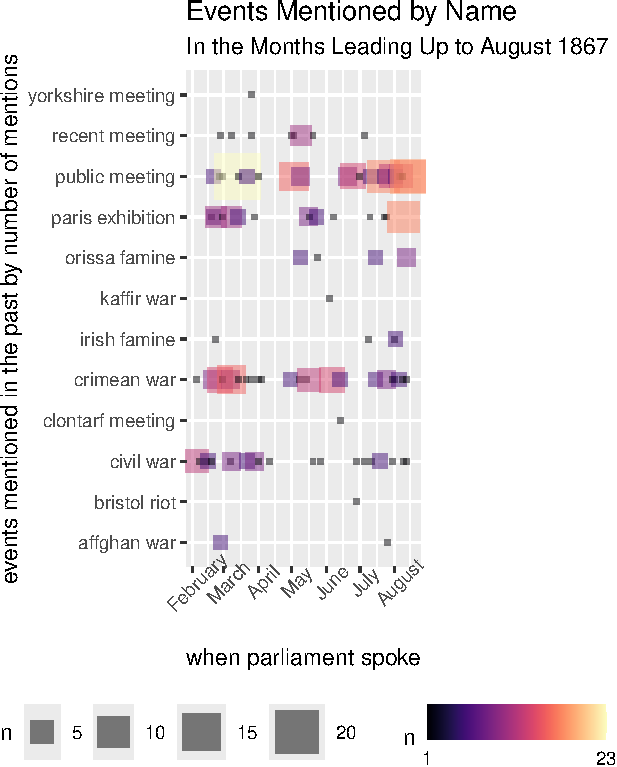
\includegraphics[keepaspectratio]{ch2_files/figure-latex/unnamed-chunk-26-1.pdf}}
\caption{Plot showing the frequency with which Parliament in 1867
referred to major past events---including famines, wars, riots, and
public meetings---across the months from February to August. Each square
represents a day on which a speech mentioned a given event bigram;
larger and brighter squares indicate higher numbers of mentions.}
\end{figure}

What do we make of this timeline? It suggests a swell of public meetings
referenced in parliament in the months leading up to August 1867, which
received more intense attention than either the Crimean War or the Paris
Exhibition. Individual meetings such as those in Yorkshire or Clontarf
received passing acknowledgment rather than deeper debate. Understanding
the results of the visualization deeper requires more cycles of research
and reading.

Other research questions appear that the individual analyst, engaged in
a process of research, would want to follow. Did references to public
meetings change from January to August, while their mentions
intensified? Were all of these public meetings about the vote? What was
the meaning of references to a ``civil war'' -- the English civil war or
recent events in America -- and was this civil war invoked in reference
to 1867? What about the references to the contemporary famine in Orissa
(in India) or the (presumably historical) famine in Ireland?

One way to approach this line of inquiry would be by using the graph we
have generated as a source of concrete questions about how members of
parliament invoked current and historical events in the lead-up to the
vote on the Second Reform Act. An analyst of history would follow up on
most of these questions by reading individual sentences, speeches, and
entire debates and to form these readings into a historical argument
about the role of events in shaping political reform.

\subsection{Finding Historical Events Using a Controlled
Vocabulary}\label{finding-historical-events-using-a-controlled-vocabulary}

Next, let's return to the idea of finding events using what we have
learned about joins. The authors of this book have created a controlled
vocabulary of event names which lists the date of famous events like the
Magna Carta (1215).

As \emph{The Dangerous Art of Text Mining} makes clear, we understand
that there is no universal definition of the most important events in
world history. Any controlled vocabulary list has its merits and its
omissions. It is in comparing the subtleties of different lists of
events that the historian begins to explore the changing political and
cultural nature of memory -- for example, the fact that references to
the Glorious Revolution began to disappear after the First Reform Act,
gradually displaced by allusions to the Tudor past.

\begin{Shaded}
\begin{Highlighting}[]
\CommentTok{\# load the scholar{-}created "events" dataset from hansardr}
\FunctionTok{data}\NormalTok{(}\StringTok{"events"}\NormalTok{)}

\CommentTok{\# process the dataset to get a cleaned list of historical events}
\CommentTok{\# each row represents a unique event with its assigned historical date}
\CommentTok{\# ensures lowercase names for matching and excludes events after 1840}
\NormalTok{eventslist }\OtherTok{\textless{}{-}}\NormalTok{ events }\SpecialCharTok{\%\textgreater{}\%} \CommentTok{\# create a new dataset}
  \FunctionTok{distinct}\NormalTok{(event\_name, scholar\_assigned\_date) }\SpecialCharTok{\%\textgreater{}\%} \CommentTok{\# remove duplicates}
  \FunctionTok{filter}\NormalTok{(}\SpecialCharTok{!}\NormalTok{scholar\_assigned\_date }\SpecialCharTok{\textgreater{}} \DecValTok{1840}\NormalTok{) }\SpecialCharTok{\%\textgreater{}\%} \CommentTok{\# exclude post{-}1840 events}
  \FunctionTok{mutate}\NormalTok{(}\AttributeTok{event\_name =} \FunctionTok{tolower}\NormalTok{(event\_name)) }\SpecialCharTok{\%\textgreater{}\%} \CommentTok{\# lowercase event names}
  \FunctionTok{select}\NormalTok{(event\_name, scholar\_assigned\_date) }\CommentTok{\# keep only name and date}

\FunctionTok{head}\NormalTok{(eventslist)}
\end{Highlighting}
\end{Shaded}

\begin{verbatim}
## # A tibble: 6 x 2
##   event_name          scholar_assigned_date
##   <chr>                               <dbl>
## 1 french revolution                    1789
## 2 magna carta                          1215
## 3 norman conquest                      1066
## 4 corn laws                            1815
## 5 battle of boyne                      1690
## 6 glorious revolution                  1688
\end{verbatim}

Notice that events contains two columns: events by their name, and the
historical dates on which those events occurred.

We will now count events mentioned in parliamentary speeches, starting
with using an \texttt{inner\_join()}. Like its cousin,
\texttt{left\_join()}, \texttt{inner\_join()} works with two data sets
to make a new, combined data set. We use \texttt{inner\_join()} when we
want to analyze shared areas of overlap between two data sets. For our
analysis. we want to find the n-grams from \texttt{annotated\_1830} that
are also listed as entities in the events controlled vocabulary.

\begin{Shaded}
\begin{Highlighting}[]
\CommentTok{\# Load the Hansard speech text and associated metadata for the year 1830}
\FunctionTok{data}\NormalTok{(}\StringTok{"hansard\_1830"}\NormalTok{)}
\FunctionTok{data}\NormalTok{(}\StringTok{"debate\_metadata\_1830"}\NormalTok{)}

\CommentTok{\# Merge the speech data with its metadata using a left join}
\CommentTok{\# All rows from hansard\_1830 are retained, with metadata added where available}
\NormalTok{hansard\_1830 }\OtherTok{\textless{}{-}}\NormalTok{ hansard\_1830 }\SpecialCharTok{\%\textgreater{}\%} \CommentTok{\# create a new dataset}
  \FunctionTok{left\_join}\NormalTok{(debate\_metadata\_1830) }\CommentTok{\# join debate text and metadata}

\CommentTok{\# Tokenize the speech text into bigrams}
\CommentTok{\# {-} "ngram" is the name of the new column to store the bigrams}
\CommentTok{\# {-} "text" is the input column containing the speech text}
\CommentTok{\# {-} token = "ngrams" with n = 2 instructs the function to extract bigrams}
\NormalTok{bigrams\_1830 }\OtherTok{\textless{}{-}}\NormalTok{ hansard\_1830 }\SpecialCharTok{\%\textgreater{}\%} \CommentTok{\# create a new dataset}
  \FunctionTok{unnest\_tokens}\NormalTok{(ngram, text, }\AttributeTok{token =} \StringTok{"ngrams"}\NormalTok{, }\AttributeTok{n =} \DecValTok{2}\NormalTok{) }\CommentTok{\# tokenize text column}

\CommentTok{\# Identify bigrams that match known historical events from "eventslist"}
\CommentTok{\# {-} Performs an inner join where the bigram matches the cleaned event name}
\CommentTok{\# {-} Keeps only rows with a match, linking bigram use to historical context}
\NormalTok{events\_1830 }\OtherTok{\textless{}{-}}\NormalTok{ bigrams\_1830 }\SpecialCharTok{\%\textgreater{}\%} \CommentTok{\# create a new dataset}
  \FunctionTok{inner\_join}\NormalTok{(eventslist, }\AttributeTok{by =} \FunctionTok{c}\NormalTok{(}\StringTok{"ngram"} \OtherTok{=} \StringTok{"event\_name"}\NormalTok{)) }\CommentTok{\# join the bigrams and events}

\NormalTok{events\_1830 }\SpecialCharTok{\%\textgreater{}\%}
  \FunctionTok{head}\NormalTok{() }\SpecialCharTok{\%\textgreater{}\%}
  \FunctionTok{mutate}\NormalTok{(}\AttributeTok{ngram =} \FunctionTok{str\_trunc}\NormalTok{(ngram, }\DecValTok{120}\NormalTok{)) }\SpecialCharTok{\%\textgreater{}\%}  
  \FunctionTok{kable}\NormalTok{(}\AttributeTok{format =} \StringTok{"latex"}\NormalTok{, }
        \AttributeTok{booktabs =} \ConstantTok{TRUE}\NormalTok{,}
        \AttributeTok{caption =} \StringTok{"Sample two{-}word phrase events from the 1830 Hansard debates."}\NormalTok{) }\SpecialCharTok{\%\textgreater{}\%}
  \FunctionTok{kable\_styling}\NormalTok{(}\AttributeTok{full\_width =} \ConstantTok{FALSE}\NormalTok{,}
                \AttributeTok{position =} \StringTok{"left"}\NormalTok{,}
                \AttributeTok{latex\_options =} \FunctionTok{c}\NormalTok{(}\StringTok{"hold\_position"}\NormalTok{, }\StringTok{"scale\_down"}\NormalTok{),}
                \AttributeTok{font\_size =} \DecValTok{7}\NormalTok{) }\SpecialCharTok{\%\textgreater{}\%} 
  \FunctionTok{column\_spec}\NormalTok{(}\DecValTok{3}\NormalTok{, }\AttributeTok{width =} \StringTok{"4cm"}\NormalTok{)}
\end{Highlighting}
\end{Shaded}

\begin{table}[!h]

\caption{\label{tab:unnamed-chunk-28}Sample two-word phrase events from the 1830 Hansard debates.}
\resizebox{\ifdim\width>\linewidth\linewidth\else\width\fi}{!}{
\fontsize{7}{9}\selectfont
\begin{tabular}[t]{ll>{\raggedright\arraybackslash}p{4cm}lr}
\toprule
sentence\_id & speechdate & debate & ngram & scholar\_assigned\_date\\
\midrule
S2V0022P0\_158 & 1830-02-04 & ADDRESS ON THE LORDS COMMISSIONERS SPEECH. ] & navigation laws & 1660\\
S2V0022P0\_1722 & 1830-02-18 & POUTUGAL. ] & portuguese constitution & 1822\\
S2V0022P0\_1729 & 1830-02-18 & POUTUGAL. ] & portuguese constitution & 1822\\
S2V0022P0\_1735 & 1830-02-18 & POUTUGAL. ] & portuguese constitution & 1822\\
S2V0022P0\_1833 & 1830-02-18 & POUTUGAL. ] & portuguese constitution & 1822\\
\addlinespace
S2V0022P0\_1923 & 1830-02-18 & POUTUGAL. ] & portuguese constitution & 1822\\
\bottomrule
\end{tabular}}
\end{table}

Notice that the resulting dataset contains speaker and date columns from
the parliamentary speeches, but the only bigrams listed are those that
correspond to events from \texttt{eventslist}.

In the next blocks of code, we use our new list of events to generate a
visualization.

\begin{Shaded}
\begin{Highlighting}[]
\CommentTok{\# count how many times each event bigram is mentioned on each speech date}
\CommentTok{\# extract year from date, group by relevant fields, and remove grouping after summarizing}
\NormalTok{counted\_events }\OtherTok{\textless{}{-}}\NormalTok{ events\_1830 }\SpecialCharTok{\%\textgreater{}\%} \CommentTok{\# create a new dataset}
  \FunctionTok{mutate}\NormalTok{(}\AttributeTok{year =} \FunctionTok{year}\NormalTok{(speechdate)) }\SpecialCharTok{\%\textgreater{}\%} \CommentTok{\# extract year from speech date}
  \FunctionTok{group\_by}\NormalTok{(ngram, year, speechdate, scholar\_assigned\_date) }\SpecialCharTok{\%\textgreater{}\%} \CommentTok{\# group data}
  \FunctionTok{summarize}\NormalTok{(}\AttributeTok{n =} \FunctionTok{n}\NormalTok{()) }\SpecialCharTok{\%\textgreater{}\%} \CommentTok{\# count mentions}
  \FunctionTok{ungroup}\NormalTok{() }\CommentTok{\# remove grouping}

\FunctionTok{head}\NormalTok{(counted\_events)}
\end{Highlighting}
\end{Shaded}

\begin{verbatim}
## # A tibble: 6 x 5
##   ngram                  year speechdate scholar_assigned_date     n
##   <chr>                 <dbl> <IDate>                    <dbl> <int>
## 1 american constitution  1831 1831-10-05                  1776     1
## 2 american constitution  1831 1831-10-06                  1776     2
## 3 american constitution  1832 1832-04-13                  1776     2
## 4 belgian revolution     1831 1831-08-09                  1830     1
## 5 belgian revolution     1831 1831-08-18                  1830     1
## 6 belgian revolution     1832 1832-03-16                  1830    10
\end{verbatim}

\begin{Shaded}
\begin{Highlighting}[]
\CommentTok{\# summarize total mentions of each event across all speech dates}
\CommentTok{\# grouped by event name and assigned historical date}
\CommentTok{\# then sort chronologically for historical analysis}
\NormalTok{cleaned\_events }\OtherTok{\textless{}{-}}\NormalTok{ counted\_events }\SpecialCharTok{\%\textgreater{}\%}
  \FunctionTok{group\_by}\NormalTok{(ngram, scholar\_assigned\_date) }\SpecialCharTok{\%\textgreater{}\%} \CommentTok{\# group by event and historical date}
  \FunctionTok{summarize}\NormalTok{(}\AttributeTok{total =} \FunctionTok{sum}\NormalTok{(n)) }\SpecialCharTok{\%\textgreater{}\%} \CommentTok{\# sum total mentions}
  \FunctionTok{ungroup}\NormalTok{() }\SpecialCharTok{\%\textgreater{}\%} \CommentTok{\# remove grouping}
  \FunctionTok{arrange}\NormalTok{(scholar\_assigned\_date) }\CommentTok{\# sort by historical date}

\FunctionTok{head}\NormalTok{(cleaned\_events)}
\end{Highlighting}
\end{Shaded}

\begin{verbatim}
## # A tibble: 6 x 3
##   ngram              scholar_assigned_date total
##   <chr>                              <dbl> <int>
## 1 norman conquest                     1066     5
## 2 twelfth century                     1100     3
## 3 thirteenth century                  1200     7
## 4 fourteenth century                  1300     2
## 5 game laws                           1389   112
## 6 fifteenth century                   1400     7
\end{verbatim}

\begin{Shaded}
\begin{Highlighting}[]
\CommentTok{\# create an index to divide the historical date range into 30 equal chronological bins}
\CommentTok{\# group by each bin and select the most frequently mentioned event within each}
\CommentTok{\# then join back with the full event data to recover speech{-}level detail}
\NormalTok{indexed\_events }\OtherTok{\textless{}{-}}\NormalTok{ cleaned\_events }\SpecialCharTok{\%\textgreater{}\%}
  \FunctionTok{mutate}\NormalTok{(}\AttributeTok{index =}\NormalTok{ scholar\_assigned\_date }\SpecialCharTok{\%/\%} 
\NormalTok{           ((}\FunctionTok{max}\NormalTok{(scholar\_assigned\_date) }\SpecialCharTok{{-}} 
               \FunctionTok{min}\NormalTok{(scholar\_assigned\_date)) }\SpecialCharTok{/} \DecValTok{30}\NormalTok{)) }\SpecialCharTok{\%\textgreater{}\%} \CommentTok{\# assign bin index}
  \FunctionTok{group\_by}\NormalTok{(index) }\SpecialCharTok{\%\textgreater{}\%} \CommentTok{\# group by time bin}
  \FunctionTok{filter}\NormalTok{(total }\SpecialCharTok{==} \FunctionTok{max}\NormalTok{(total)) }\SpecialCharTok{\%\textgreater{}\%} \CommentTok{\# keep most mentioned event in each bin}
  \FunctionTok{ungroup}\NormalTok{() }\SpecialCharTok{\%\textgreater{}\%} \CommentTok{\# remove grouping}
  \FunctionTok{left\_join}\NormalTok{(counted\_events, }\AttributeTok{by =} \FunctionTok{c}\NormalTok{(}\StringTok{"ngram"}\NormalTok{, }\StringTok{"scholar\_assigned\_date"}\NormalTok{)) }\CommentTok{\# join data}

\FunctionTok{head}\NormalTok{(indexed\_events)}
\end{Highlighting}
\end{Shaded}

\begin{verbatim}
## # A tibble: 6 x 7
##   ngram           scholar_assigned_date total index  year speechdate     n
##   <chr>                           <dbl> <int> <dbl> <dbl> <IDate>    <int>
## 1 norman conquest                  1066     5    41  1830 1830-11-15     1
## 2 norman conquest                  1066     5    41  1834 1834-03-14     1
## 3 norman conquest                  1066     5    41  1834 1834-04-25     1
## 4 norman conquest                  1066     5    41  1839 1839-07-12     2
## 5 twelfth century                  1100     3    43  1831 1831-07-06     1
## 6 twelfth century                  1100     3    43  1832 1832-02-27     1
\end{verbatim}

\begin{Shaded}
\begin{Highlighting}[]
\CommentTok{\# Define a boundary value by adding 8 days to the latest speech date in the dataset}
\CommentTok{\# Make the visualization easier to read by adding padding to the visualization}
\NormalTok{left\_range }\OtherTok{\textless{}{-}} \FunctionTok{max}\NormalTok{(events\_1830}\SpecialCharTok{$}\NormalTok{speechdate) }\SpecialCharTok{+} \DecValTok{8}
\end{Highlighting}
\end{Shaded}

\begin{Shaded}
\begin{Highlighting}[]
\CommentTok{\# create a bubble plot showing when historical events were mentioned in parliament}
\CommentTok{\# x{-}axis shows the date of mention; y{-}axis shows the historical date of the event}
\CommentTok{\# bubble size and color represent frequency of mentions}
\FunctionTok{ggplot}\NormalTok{(}\AttributeTok{data =}\NormalTok{ indexed\_events, }\CommentTok{\# provide the name of the dataset}
       \FunctionTok{aes}\NormalTok{(}\AttributeTok{x =}\NormalTok{ speechdate, }\CommentTok{\# assign the x{-}axis}
           \AttributeTok{y =}\NormalTok{ scholar\_assigned\_date, }\CommentTok{\# assign the y{-}axis}
           \AttributeTok{size =}\NormalTok{ n, }\CommentTok{\# assign the size of the points}
           \AttributeTok{label =} \FunctionTok{paste0}\NormalTok{(}\StringTok{"            "}\NormalTok{, ngram, }\StringTok{" ("}\NormalTok{, scholar\_assigned\_date, }\StringTok{")"}\NormalTok{),}
           \AttributeTok{color =}\NormalTok{ n)) }\SpecialCharTok{+}  \CommentTok{\# assign the color}

\CommentTok{\# use viridis color scale with log transform for better contrast}
\CommentTok{\# set bubble size aesthetics for visual clarity}
\CommentTok{\# use viridis option A (purple to yellow{-}green gradient)}
\CommentTok{\# and use a forward gradient (low values = dark, high = bright)}
  \FunctionTok{scale\_color\_viridis}\NormalTok{(}\AttributeTok{breaks =}\NormalTok{ round, }\CommentTok{\# round legend breaks}
                    \AttributeTok{trans =} \StringTok{"log"}\NormalTok{, }\CommentTok{\# log scale}
                    \AttributeTok{option =} \StringTok{"A"}\NormalTok{, }\CommentTok{\# viridis option}
                    \AttributeTok{discrete =} \ConstantTok{FALSE}\NormalTok{, }\CommentTok{\# continuous scale}
                    \AttributeTok{direction =} \DecValTok{1}\NormalTok{) }\SpecialCharTok{+} \CommentTok{\# forward gradient}

  \CommentTok{\# set up point appearance, plot boundaries, and x{-}axis formatting}
  \CommentTok{\# this controls how bubbles are sized, shaped, placed, and how time is shown}
  \FunctionTok{scale\_size\_continuous}\NormalTok{(}\AttributeTok{range =} \FunctionTok{c}\NormalTok{(}\DecValTok{1}\NormalTok{, }\DecValTok{10}\NormalTok{)) }\SpecialCharTok{+} \CommentTok{\# bubble size range}
  \FunctionTok{geom\_point}\NormalTok{(}\AttributeTok{alpha =}\NormalTok{ .}\DecValTok{5}\NormalTok{, }\AttributeTok{shape =} \DecValTok{15}\NormalTok{) }\SpecialCharTok{+} \CommentTok{\# square bubbles}
  \FunctionTok{coord\_cartesian}\NormalTok{(}\AttributeTok{clip =} \StringTok{"off"}\NormalTok{) }\SpecialCharTok{+} \CommentTok{\# no clipping of labels}
  \FunctionTok{scale\_x\_date}\NormalTok{(}\AttributeTok{date\_breaks =} \StringTok{"1 year"}\NormalTok{, }\AttributeTok{date\_labels =} \StringTok{"\%Y"}\NormalTok{) }\SpecialCharTok{+} \CommentTok{\# yearly ticks on x{-}axis}

  \CommentTok{\# add one label per event, placed at the right edge and aligned with its historical date}
  \FunctionTok{geom\_text}\NormalTok{(}\AttributeTok{data =}\NormalTok{ indexed\_events }\SpecialCharTok{\%\textgreater{}\%} \CommentTok{\# assign data}
            \FunctionTok{group\_by}\NormalTok{(ngram) }\SpecialCharTok{\%\textgreater{}\%} \CommentTok{\# group data}
            \FunctionTok{sample\_n}\NormalTok{(}\DecValTok{1}\NormalTok{), }\CommentTok{\# pick one speech instance per event}
            \AttributeTok{show.legend =} \ConstantTok{FALSE}\NormalTok{, }\CommentTok{\# no text in legend}
            \FunctionTok{aes}\NormalTok{(}\AttributeTok{color =} \DecValTok{1}\NormalTok{, }\CommentTok{\# fixed color for all labels}
                \AttributeTok{x =}\NormalTok{ left\_range, }\CommentTok{\# position label at far right}
                \AttributeTok{y =}\NormalTok{ scholar\_assigned\_date, }\CommentTok{\# align vertically with event date}
                \AttributeTok{hjust =} \DecValTok{0}\NormalTok{, }\CommentTok{\# left{-}align label text}
                \AttributeTok{size =} \DecValTok{8}\NormalTok{)) }\SpecialCharTok{+} \CommentTok{\# label size}

  \CommentTok{\# style plot appearance for readability and layout}
  \FunctionTok{theme}\NormalTok{(}\AttributeTok{legend.position =} \StringTok{"bottom"}\NormalTok{, }\CommentTok{\# move legend below plot}
        \AttributeTok{plot.margin =} \FunctionTok{unit}\NormalTok{(}\FunctionTok{c}\NormalTok{(}\DecValTok{1}\NormalTok{, }\DecValTok{250}\NormalTok{, }\DecValTok{50}\NormalTok{, }\DecValTok{1}\NormalTok{), }\AttributeTok{unit =} \StringTok{"pt"}\NormalTok{), }\CommentTok{\# add right margin for labels}
        \AttributeTok{axis.text.x =} \FunctionTok{element\_text}\NormalTok{(}\AttributeTok{angle =} \DecValTok{45}\NormalTok{, }\AttributeTok{vjust =} \FloatTok{0.5}\NormalTok{, }\AttributeTok{hjust =} \DecValTok{1}\NormalTok{), }\CommentTok{\# rotate x{-}axis labels}
        \AttributeTok{axis.title.x =} \FunctionTok{element\_text}\NormalTok{(}\AttributeTok{vjust =} \SpecialCharTok{{-}}\FloatTok{0.5}\NormalTok{)) }\SpecialCharTok{+} \CommentTok{\# adjust x{-}axis title spacing}
  \FunctionTok{guides}\NormalTok{(}\AttributeTok{shape =} \StringTok{"none"}\NormalTok{) }\SpecialCharTok{+} \CommentTok{\# remove shape legend}

  \CommentTok{\# add axis labels and title}
  \FunctionTok{labs}\NormalTok{(}\AttributeTok{x =} \StringTok{"when parliament spoke"}\NormalTok{, }\CommentTok{\# assign the x{-}axis}
       \AttributeTok{y =} \StringTok{"events mentioned in the past"}\NormalTok{) }\SpecialCharTok{+} \CommentTok{\# assign the y{-}axis}
  \FunctionTok{ggtitle}\NormalTok{(}\StringTok{"Events Mentioned by Name in Parliament"}\NormalTok{) }\CommentTok{\# create a title}
\end{Highlighting}
\end{Shaded}

\begin{figure}
\centering
\pandocbounded{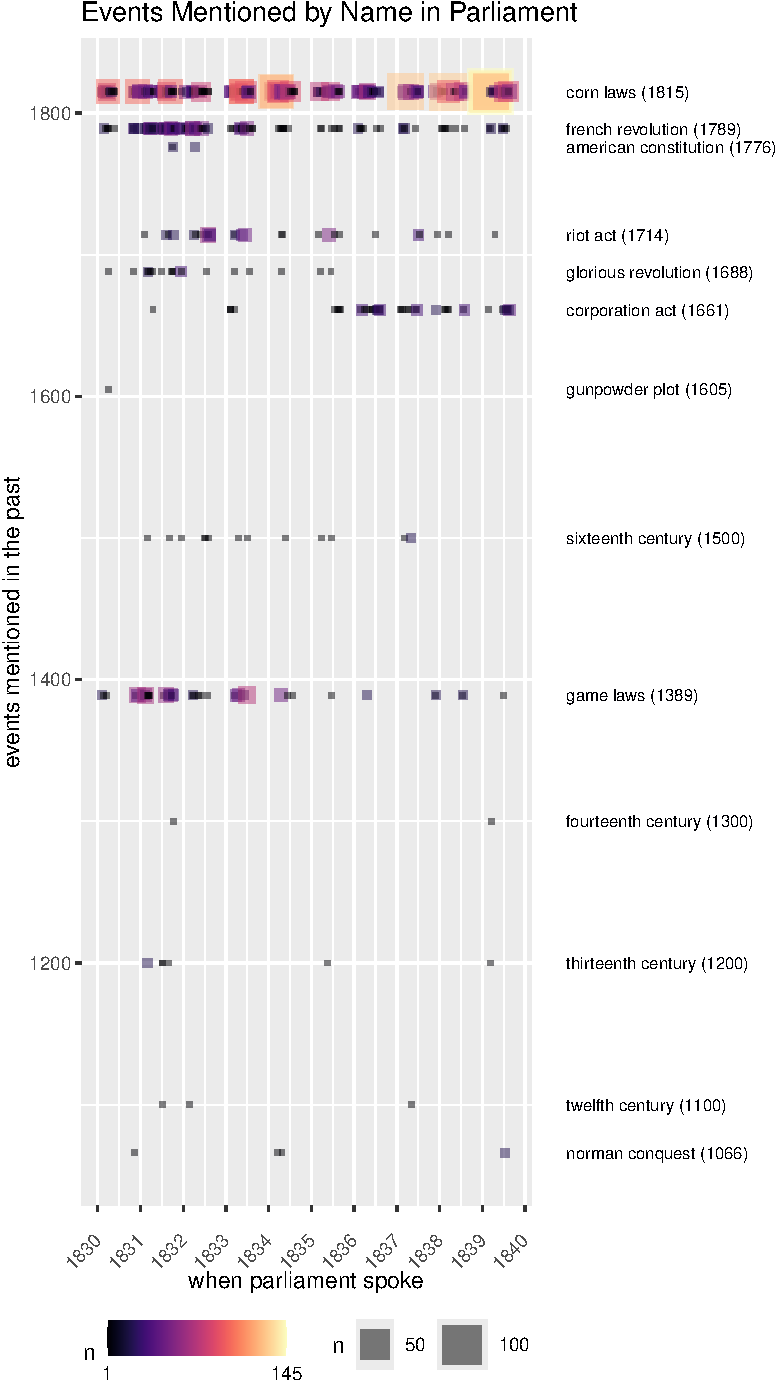
\includegraphics[keepaspectratio]{ch2_files/figure-latex/unnamed-chunk-33-1.pdf}}
\caption{Plot of how often nineteenth-century MPs invoked earlier
historical events in the debates of the 1830s. The x-axis shows when
speeches were delivered (1830--1840), while the y-axis shows the
historical date of the event being named. Each square marks at least one
speech mentioning that event; larger and brighter squares indicate more
frequent references, highlighting especially intensive discussion of
late eighteenth- and early nineteenth-century events such as the Corn
Laws, the French Revolution, and the American Constitution.}
\end{figure}

Note that the visualization here resembles the visualization of events
we generated above, but in this case, we have some extra information:
the actual date of the event mentioned, e.g.~1789 for the French
Revolution. We have plotted this historical information on the y-axis.
The resulting graph in fact shows two timelines rather than one -- a
timeline of parliamentary speech on the x-axis and a timeline of
historical references on the y-axis.

How should we interpret this graph? One approach is to identify the most
surprising aspects of the visualization and explore their implications.
For instance, as a British historian, I am unsurprised by frequent
references in Parliament to events from the previous half-century, such
as the French and American Revolutions. Similarly, it's expected that
the Glorious Revolution was heavily referenced in the early 1830s, with
mentions tapering off after 1836, and that the Riot Act was invoked
annually. However, the most striking feature of the graph may be the
vertical line around 1832, where references to much older historical
periods---the sixteenth, thirteenth, and twelfth centuries---appear.
This invocation of the distant past invites further investigation into
its context and significance.

Why? we find ourselves asking. That verticality of temporal
experience--the long perspective on the deep past--seems to be fairly
distinct for 1830-32 of all the years in the decade. Why do so many
different, varied periods suddenly become relevant all at once? Is this
pattern a general characteristic of moments of political reform -- that
the deep past is trawled for a multitude of examples, for and against?

We continue the explanation through reading.

\begin{Shaded}
\begin{Highlighting}[]
\CommentTok{\# add a new column extracting the year from the speech date}
\NormalTok{hansard\_1830 }\OtherTok{\textless{}{-}}\NormalTok{ hansard\_1830 }\SpecialCharTok{\%\textgreater{}\%}
  \FunctionTok{mutate}\NormalTok{(}\AttributeTok{year =} \FunctionTok{year}\NormalTok{(speechdate))}

\CommentTok{\# filter speeches from the year 1832 that mention the phrase "fifteenth century"}
\CommentTok{\# {-} str\_detect() searches for the exact phrase in the text}
\CommentTok{\# {-} select() keeps only the "text" column of the matching speeches}
\NormalTok{c15\_mentions }\OtherTok{\textless{}{-}}\NormalTok{ hansard\_1830 }\SpecialCharTok{\%\textgreater{}\%} \CommentTok{\# create a new dataset}
  \FunctionTok{filter}\NormalTok{(year }\SpecialCharTok{\textgreater{}} \DecValTok{1831} \SpecialCharTok{\&}\NormalTok{ year }\SpecialCharTok{\textless{}} \DecValTok{1833}\NormalTok{, }\CommentTok{\# filter for the date range}
         \FunctionTok{str\_detect}\NormalTok{(text, }\StringTok{"fifteenth century"}\NormalTok{)) }\SpecialCharTok{\%\textgreater{}\%} \CommentTok{\# detect the phrase}
  \FunctionTok{select}\NormalTok{(text) }\CommentTok{\# select just the text column}
\end{Highlighting}
\end{Shaded}

\begin{Shaded}
\begin{Highlighting}[]
\NormalTok{c15\_mentions }\SpecialCharTok{\%\textgreater{}\%}
  \FunctionTok{head}\NormalTok{() }\SpecialCharTok{\%\textgreater{}\%}
  \FunctionTok{mutate}\NormalTok{(}\AttributeTok{text =} \FunctionTok{str\_wrap}\NormalTok{(text, }\DecValTok{80}\NormalTok{)) }\SpecialCharTok{\%\textgreater{}\%}
  \FunctionTok{select}\NormalTok{(text) }\SpecialCharTok{\%\textgreater{}\%}
  \FunctionTok{kable}\NormalTok{(}\AttributeTok{format =} \StringTok{"latex"}\NormalTok{, }
        \AttributeTok{booktabs =} \ConstantTok{TRUE}\NormalTok{, }
        \AttributeTok{longtable =} \ConstantTok{TRUE}\NormalTok{, }
        \AttributeTok{escape =} \ConstantTok{FALSE}\NormalTok{,}
        \AttributeTok{caption =} \StringTok{""}\NormalTok{) }\SpecialCharTok{\%\textgreater{}\%}
  \FunctionTok{column\_spec}\NormalTok{(}\DecValTok{1}\NormalTok{, }\AttributeTok{width =} \StringTok{"14cm"}\NormalTok{)}
\end{Highlighting}
\end{Shaded}

\begin{longtable}[t]{>{\raggedright\arraybackslash}p{14cm}}
\caption{\label{tab:unnamed-chunk-35}}\\
\toprule
text\\
\midrule
The celebrated Act of William (1696) was only a transcript from a Scottish
law of the fifteenth century, which was itself the enforcement only, by civil
sanction, of the original canon of the Catholic Church.\\
\bottomrule
\end{longtable}

\begin{Shaded}
\begin{Highlighting}[]
\CommentTok{\# Filter speeches from the year 1832 that mention the phrase "fourteenth century"}
\CommentTok{\# {-} Only rows with "fourteenth century" in the text are retained}
\CommentTok{\# {-} Only the "text" column is selected}
\NormalTok{c14\_mentions }\OtherTok{\textless{}{-}}\NormalTok{ hansard\_1830 }\SpecialCharTok{\%\textgreater{}\%} \CommentTok{\# create a new dataset}
  \FunctionTok{filter}\NormalTok{(year }\SpecialCharTok{\textgreater{}} \DecValTok{1831} \SpecialCharTok{\&}\NormalTok{ year }\SpecialCharTok{\textless{}} \DecValTok{1833}\NormalTok{, }\CommentTok{\# filter for the date range}
         \FunctionTok{str\_detect}\NormalTok{(text, }\StringTok{"fourteenth century"}\NormalTok{)) }\SpecialCharTok{\%\textgreater{}\%} \CommentTok{\# detect the phrase}
  \FunctionTok{select}\NormalTok{(text) }\CommentTok{\# select just the text column}
\end{Highlighting}
\end{Shaded}

\begin{Shaded}
\begin{Highlighting}[]
\CommentTok{\# display the filtered speech texts that mention "fourteenth century"}
\NormalTok{c14\_mentions }\SpecialCharTok{\%\textgreater{}\%}
  \FunctionTok{head}\NormalTok{() }\SpecialCharTok{\%\textgreater{}\%}
  \FunctionTok{mutate}\NormalTok{(}\AttributeTok{text =} \FunctionTok{str\_wrap}\NormalTok{(text, }\DecValTok{80}\NormalTok{)) }\SpecialCharTok{\%\textgreater{}\%}
  \FunctionTok{select}\NormalTok{(text) }\SpecialCharTok{\%\textgreater{}\%}
  \FunctionTok{kable}\NormalTok{(}\StringTok{"latex"}\NormalTok{, }\AttributeTok{booktabs =} \ConstantTok{TRUE}\NormalTok{, }\AttributeTok{longtable =} \ConstantTok{TRUE}\NormalTok{, }\AttributeTok{escape =} \ConstantTok{FALSE}\NormalTok{) }\SpecialCharTok{\%\textgreater{}\%}
  \FunctionTok{column\_spec}\NormalTok{(}\DecValTok{1}\NormalTok{, }\AttributeTok{width =} \StringTok{"14cm"}\NormalTok{)}
\end{Highlighting}
\end{Shaded}

\begin{longtable}{>{\raggedright\arraybackslash}p{14cm}}
\toprule
text\\


\bottomrule
\end{longtable}

\begin{Shaded}
\begin{Highlighting}[]
\CommentTok{\# Filter speeches from the year 1832 that mention the phrase "thirteenth century"}
\CommentTok{\# {-} year \textgreater{} 1831 \& year \textless{} 1833 captures only the year 1832}
\CommentTok{\# {-} str\_detect() looks for the exact phrase "thirteenth century" in the text}
\CommentTok{\# {-} select() keeps only the "text" column of matching speeches}
\NormalTok{c13\_mentions }\OtherTok{\textless{}{-}}\NormalTok{ hansard\_1830 }\SpecialCharTok{\%\textgreater{}\%} \CommentTok{\# create a new dataset}
  \FunctionTok{filter}\NormalTok{(year }\SpecialCharTok{\textgreater{}} \DecValTok{1831} \SpecialCharTok{\&}\NormalTok{ year }\SpecialCharTok{\textless{}} \DecValTok{1833}\NormalTok{, }\CommentTok{\# filter for the date range}
         \FunctionTok{str\_detect}\NormalTok{(text, }\StringTok{"thirteenth century"}\NormalTok{)) }\SpecialCharTok{\%\textgreater{}\%} \CommentTok{\# detect the phrase}
  \FunctionTok{select}\NormalTok{(text) }\CommentTok{\# select just the text column}
\end{Highlighting}
\end{Shaded}

\begin{Shaded}
\begin{Highlighting}[]
\CommentTok{\# display the filtered speech texts that mention "thirteenth century"}
\NormalTok{c13\_mentions }\SpecialCharTok{\%\textgreater{}\%}
  \FunctionTok{head}\NormalTok{() }\SpecialCharTok{\%\textgreater{}\%}
  \FunctionTok{mutate}\NormalTok{(}\AttributeTok{text =} \FunctionTok{str\_wrap}\NormalTok{(text, }\DecValTok{80}\NormalTok{)) }\SpecialCharTok{\%\textgreater{}\%}
  \FunctionTok{select}\NormalTok{(text) }\SpecialCharTok{\%\textgreater{}\%}
  \FunctionTok{kable}\NormalTok{(}\StringTok{"latex"}\NormalTok{, }\AttributeTok{booktabs =} \ConstantTok{TRUE}\NormalTok{, }\AttributeTok{longtable =} \ConstantTok{TRUE}\NormalTok{, }\AttributeTok{escape =} \ConstantTok{FALSE}\NormalTok{) }\SpecialCharTok{\%\textgreater{}\%}
  \FunctionTok{column\_spec}\NormalTok{(}\DecValTok{1}\NormalTok{, }\AttributeTok{width =} \StringTok{"14cm"}\NormalTok{)}
\end{Highlighting}
\end{Shaded}

\begin{longtable}{>{\raggedright\arraybackslash}p{14cm}}
\toprule
text\\


\bottomrule
\end{longtable}

\begin{Shaded}
\begin{Highlighting}[]
\CommentTok{\# filter speeches from the year 1832 that mention the phrase "twelfth century"}
\CommentTok{\# {-} str\_detect() searches for the exact phrase in the "text" column}
\CommentTok{\# {-} select() keeps only the "text" column}
\NormalTok{c12\_mentions }\OtherTok{\textless{}{-}}\NormalTok{ hansard\_1830 }\SpecialCharTok{\%\textgreater{}\%} \CommentTok{\# create a new dataset}
  \FunctionTok{filter}\NormalTok{(year }\SpecialCharTok{\textgreater{}} \DecValTok{1831} \SpecialCharTok{\&}\NormalTok{ year }\SpecialCharTok{\textless{}} \DecValTok{1833}\NormalTok{, }\CommentTok{\# filter for the date range}
         \FunctionTok{str\_detect}\NormalTok{(text, }\StringTok{"twelfth century"}\NormalTok{)) }\SpecialCharTok{\%\textgreater{}\%} \CommentTok{\# detect the phrase}
  \FunctionTok{select}\NormalTok{(text) }\CommentTok{\# select just the text column}
\end{Highlighting}
\end{Shaded}

\begin{Shaded}
\begin{Highlighting}[]
\CommentTok{\# display the filtered speech texts that mention "twelfth century"}
\NormalTok{c12\_mentions }\SpecialCharTok{\%\textgreater{}\%}
  \FunctionTok{head}\NormalTok{() }\SpecialCharTok{\%\textgreater{}\%}
  \FunctionTok{mutate}\NormalTok{(}\AttributeTok{text =} \FunctionTok{str\_wrap}\NormalTok{(text, }\DecValTok{80}\NormalTok{)) }\SpecialCharTok{\%\textgreater{}\%}
  \FunctionTok{select}\NormalTok{(text) }\SpecialCharTok{\%\textgreater{}\%}
  \FunctionTok{kable}\NormalTok{(}\StringTok{"latex"}\NormalTok{, }\AttributeTok{booktabs =} \ConstantTok{TRUE}\NormalTok{, }\AttributeTok{longtable =} \ConstantTok{TRUE}\NormalTok{, }\AttributeTok{escape =} \ConstantTok{FALSE}\NormalTok{) }\SpecialCharTok{\%\textgreater{}\%}
  \FunctionTok{column\_spec}\NormalTok{(}\DecValTok{1}\NormalTok{, }\AttributeTok{width =} \StringTok{"14cm"}\NormalTok{)}
\end{Highlighting}
\end{Shaded}

\begin{longtable}{>{\raggedright\arraybackslash}p{14cm}}
\toprule
text\\
\midrule
Why, there is not now a bricklayer who falls from a ladder in England, who
cannot obtain surgical assistance, infinitely superior to that which the
sovereign of Austria could command in the twelfth century.\\
\bottomrule
\end{longtable}

What we see is a collection of historical references which serve two
purposes: one is explaining why the institutions of the past differ from
the needs of the present, and one is invoking the fact that
parliamentary institutions have changed in the past to support the cause
of reform in the present. The arguments work together, not against each
other.

While we acknowledge that other historians have studied the discourse of
parliamentary reform in detail, and even arrived at this same
conclusion, what we find from a data-driven analysis of historical
references to past events in parliament is the distinctiveness of 1832
as a moment of memory. Understanding how memory was used requires deep
reading and a knowledge of the context of the debates over the vote; but
understanding that historical memory was being leveraged in a
particularly intensive way in 1832 is an insight that comes from
treating text as data.

\subsubsection{Data Processing Order}\label{data-processing-order}

Throughout this chapter, we worked with large datasets and showed how to
handle them effectively The process we demonstrated is especially
important when handling a dataste as large the Hansard corpus. For
example, if we try to tokenize the entire dataset before narrowing it
down, the tokenization steps can exceed our computer's resources.
Instead, by first filtering the dataset to include only the debates we
care about--and then tokenizing--we can significantly reduce the
processing load.

Here is a typical workflow for handling large data like Hansard:

\begin{itemize}
\item
  Load the Dataset: Import the dataset into your R environment using
  appropriate functions like \texttt{read\_csv()}.
\item
  Filter or Subset the Dataset: Narrow down the dataset to include only
  the data relevant to your analysis. For example, if we are analyzing
  speeches by William Gladstone, we can filter rows where the speaker is
  Gladstone using functions like \texttt{filter()} from the
  \texttt{dplyr} package. Similarly, we could filter for speeches
  belonging to a specific debate by filtering the data based on a title.
  Subsetting early in the process reduces the amount of data that will
  be processed later, saving processing time and computational
  resources.
\item
  Clean the Dataset: After subsetting, clean the dataset to prepare it
  for analysis. Cleaning typically involves handling missing values,
  removing stop words, and normalizing text (e.g., converting text to
  lowercase). We can clean data with functions like \texttt{mutate()}
  from \texttt{dplyr}, or string processing functions like
  \texttt{str\_to\_lower()}, which transforms text to lower case, from
  the \texttt{stringr} package.
\item
  Analyze the Dataset: Now that you have just the needed data, perform
  your analysis by applying metrics.
\end{itemize}

Although it is poossible clean the entire dataset before narrowing it
down, doing so can strain our computer's processing power or even exceed
its available memory. It is often more desirable to filter the dataset
first, then clean the smaller, more manageable portion. Following the
order: Load -\textgreater{} Subset -\textgreater{} Clean -\textgreater{}
Analyze can optimize data processing, which may be especially useful
when analyzing change over decades or centuries of data.

\section{Exercises}\label{exercises}

\subsection{1) In the code above, we searched for 5-word phrases that
reference ``the people.'' Use the code to find two-word phrases in 1830,
1840, 1850, and 1860 that reference ``meeting.'' Write a paragraph,
quoting at least 10 phrases from each decade. For each of the phrases
mentioned more than five times, describe what prejudices, positive or
negative, the phrase encapsulates. Use your evidence to answer the
question: how did parliamentary references to meetings change between
1830 and
1860?}\label{in-the-code-above-we-searched-for-5-word-phrases-that-reference-the-people.-use-the-code-to-find-two-word-phrases-in-1830-1840-1850-and-1860-that-reference-meeting.-write-a-paragraph-quoting-at-least-10-phrases-from-each-decade.-for-each-of-the-phrases-mentioned-more-than-five-times-describe-what-prejudices-positive-or-negative-the-phrase-encapsulates.-use-your-evidence-to-answer-the-question-how-did-parliamentary-references-to-meetings-change-between-1830-and-1860}

Tips: Instead of joining every decade together, process the decades
separately to avoiding using all your computer's resources.

\begin{Shaded}
\begin{Highlighting}[]
\FunctionTok{data}\NormalTok{(}\StringTok{"hansard\_1830"}\NormalTok{)}
\FunctionTok{data}\NormalTok{(}\StringTok{"debate\_metadata\_1830"}\NormalTok{)}

\NormalTok{hansard\_1830 }\OtherTok{\textless{}{-}} \FunctionTok{left\_join}\NormalTok{(hansard\_1830, debate\_metadata\_1830, }\AttributeTok{by =} \StringTok{"sentence\_id"}\NormalTok{)}

\NormalTok{hansard\_1830\_meeting }\OtherTok{\textless{}{-}}\NormalTok{ hansard\_1830 }\SpecialCharTok{\%\textgreater{}\%} 
  \FunctionTok{mutate}\NormalTok{(}\AttributeTok{year =} \FunctionTok{year}\NormalTok{(speechdate),}
         \AttributeTok{text =} \FunctionTok{str\_to\_lower}\NormalTok{(text)) }\SpecialCharTok{\%\textgreater{}\%} 
  \FunctionTok{filter}\NormalTok{(year }\SpecialCharTok{\textgreater{}=} \DecValTok{1830}\NormalTok{, year }\SpecialCharTok{\textless{}=} \DecValTok{1839}\NormalTok{) }\SpecialCharTok{\%\textgreater{}\%}
  \FunctionTok{filter}\NormalTok{(}\FunctionTok{str\_detect}\NormalTok{(text, }\StringTok{"}\SpecialCharTok{\textbackslash{}\textbackslash{}}\StringTok{bmeetings?}\SpecialCharTok{\textbackslash{}\textbackslash{}}\StringTok{b"}\NormalTok{))}

\CommentTok{\# bigrams}
\NormalTok{bigrams\_1830 }\OtherTok{\textless{}{-}}\NormalTok{ hansard\_1830\_meeting }\SpecialCharTok{\%\textgreater{}\%}
  \FunctionTok{unnest\_tokens}\NormalTok{(bigram, text, }\AttributeTok{token =} \StringTok{"ngrams"}\NormalTok{, }\AttributeTok{n =} \DecValTok{2}\NormalTok{)}

\NormalTok{meeting\_phrases\_1830 }\OtherTok{\textless{}{-}}\NormalTok{ bigrams\_1830 }\SpecialCharTok{\%\textgreater{}\%} 
  \FunctionTok{filter}\NormalTok{(}\FunctionTok{str\_detect}\NormalTok{(bigram, }\StringTok{"\^{}[a{-}z]+ [a{-}z]+$"}\NormalTok{)) }\SpecialCharTok{\%\textgreater{}\%}
  \FunctionTok{separate}\NormalTok{(bigram, }\AttributeTok{into =} \FunctionTok{c}\NormalTok{(}\StringTok{"w1"}\NormalTok{,}\StringTok{"w2"}\NormalTok{), }\AttributeTok{sep =} \StringTok{" "}\NormalTok{, }\AttributeTok{remove =} \ConstantTok{FALSE}\NormalTok{) }\SpecialCharTok{\%\textgreater{}\%}
  \FunctionTok{filter}\NormalTok{(w1 }\SpecialCharTok{\%in\%} \FunctionTok{c}\NormalTok{(}\StringTok{"meeting"}\NormalTok{,}\StringTok{"meetings"}\NormalTok{) }\SpecialCharTok{|}\NormalTok{ w2 }\SpecialCharTok{\%in\%} \FunctionTok{c}\NormalTok{(}\StringTok{"meeting"}\NormalTok{,}\StringTok{"meetings"}\NormalTok{)) }\SpecialCharTok{\%\textgreater{}\%}
  \FunctionTok{filter}\NormalTok{(}\SpecialCharTok{!}\NormalTok{(w1 }\SpecialCharTok{\%in\%}\NormalTok{ stop\_words}\SpecialCharTok{$}\NormalTok{word }\SpecialCharTok{|}\NormalTok{ w2 }\SpecialCharTok{\%in\%}\NormalTok{ stop\_words}\SpecialCharTok{$}\NormalTok{word)) }\SpecialCharTok{\%\textgreater{}\%}
  \FunctionTok{count}\NormalTok{(bigram, }\AttributeTok{sort =} \ConstantTok{TRUE}\NormalTok{) }\SpecialCharTok{\%\textgreater{}\%}
  \FunctionTok{slice\_head}\NormalTok{(}\AttributeTok{n =} \DecValTok{80}\NormalTok{)}

\NormalTok{meeting\_phrases\_1830}
\end{Highlighting}
\end{Shaded}

\begin{verbatim}
##                   bigram   n
## 1         public meeting 410
## 2        public meetings 352
## 3           meeting held 106
## 4         county meeting  70
## 5        county meetings  42
## 6          meetings held  42
## 7         tithe meetings  33
## 8    respectable meeting  32
## 9     political meetings  31
## 10         tithe meeting  31
## 11      meeting convened  27
## 12      illegal meetings  26
## 13    protestant meeting  25
## 14          late meeting  22
## 15         meeting house  22
## 16        meeting houses  21
## 17      numerous meeting  20
## 18       illegal meeting  19
## 19   tumultuous meetings  19
## 20     political meeting  17
## 21        reform meeting  17
## 22     numerous meetings  16
## 23      private meetings  16
## 24     meeting assembled  15
## 25        meeting called  15
## 26    seditious meetings  15
## 27       private meeting  14
## 28    dissenting meeting  13
## 29       meeting alluded  12
## 30      prevent meetings  12
## 31        vestry meeting  12
## 32         house meeting  11
## 33       meeting clauses  11
## 34       vestry meetings  11
## 35    birmingham meeting  10
## 36        recent meeting  10
## 37        corner meeting   9
## 38     meetings convened   9
## 39        parish meeting   9
## 40      popular meetings   9
## 41     attended meetings   8
## 42         hold meetings   8
## 43     meeting regularly   8
## 44       reform meetings   8
## 45        annual meeting   7
## 46      holding meetings   7
## 47      intended meeting   7
## 48      meeting composed   7
## 49     meeting consisted   7
## 50     peaceable meeting   7
## 51    prohibited meeting   7
## 52       similar meeting   7
## 53      similar meetings   7
## 54         held meetings   6
## 55    meeting consisting   6
## 56      meeting recently   6
## 57        orange meeting   6
## 58        packed meeting   6
## 59       parish meetings   6
## 60       secret meetings   6
## 61 simultaneous meetings   6
## 62    attending meetings   5
## 63     chartist meetings   5
## 64         essex meeting   5
## 65     exclusive meeting   5
## 66      meeting referred   5
## 67       meetings called   5
## 68   meetings consisting   5
## 69       orange meetings   5
## 70    parochial meetings   5
## 71        party meetings   5
## 72   protestant meetings   5
## 73       special meeting   5
## 74        street meeting   5
## 75    subsequent meeting   5
## 76    tumultuous meeting   5
## 77      unlawful meeting   5
## 78       avoided meeting   4
## 79   charitable meetings   4
## 80        dublin meeting   4
\end{verbatim}

\begin{Shaded}
\begin{Highlighting}[]
\FunctionTok{data}\NormalTok{(}\StringTok{"hansard\_1840"}\NormalTok{)}
\FunctionTok{data}\NormalTok{(}\StringTok{"debate\_metadata\_1840"}\NormalTok{)}

\NormalTok{hansard\_1840 }\OtherTok{\textless{}{-}} \FunctionTok{left\_join}\NormalTok{(hansard\_1840, debate\_metadata\_1840, }\AttributeTok{by =} \StringTok{"sentence\_id"}\NormalTok{)}

\NormalTok{hansard\_1840\_meeting }\OtherTok{\textless{}{-}}\NormalTok{ hansard\_1840 }\SpecialCharTok{\%\textgreater{}\%} 
  \FunctionTok{mutate}\NormalTok{(}\AttributeTok{year =} \FunctionTok{year}\NormalTok{(speechdate),}
         \AttributeTok{text =} \FunctionTok{str\_to\_lower}\NormalTok{(text)) }\SpecialCharTok{\%\textgreater{}\%} 
  \FunctionTok{filter}\NormalTok{(year }\SpecialCharTok{\textgreater{}=} \DecValTok{1840}\NormalTok{, year }\SpecialCharTok{\textless{}=} \DecValTok{1849}\NormalTok{) }\SpecialCharTok{\%\textgreater{}\%}
  \FunctionTok{filter}\NormalTok{(}\FunctionTok{str\_detect}\NormalTok{(text, }\StringTok{"}\SpecialCharTok{\textbackslash{}\textbackslash{}}\StringTok{bmeetings?}\SpecialCharTok{\textbackslash{}\textbackslash{}}\StringTok{b"}\NormalTok{))}

\NormalTok{bigrams\_1840 }\OtherTok{\textless{}{-}}\NormalTok{ hansard\_1840\_meeting }\SpecialCharTok{\%\textgreater{}\%}
  \FunctionTok{unnest\_tokens}\NormalTok{(bigram, text, }\AttributeTok{token =} \StringTok{"ngrams"}\NormalTok{, }\AttributeTok{n =} \DecValTok{2}\NormalTok{)}

\NormalTok{meeting\_phrases\_1840 }\OtherTok{\textless{}{-}}\NormalTok{ bigrams\_1840 }\SpecialCharTok{\%\textgreater{}\%} 
  \FunctionTok{filter}\NormalTok{(}\FunctionTok{str\_detect}\NormalTok{(bigram, }\StringTok{"\^{}[a{-}z]+ [a{-}z]+$"}\NormalTok{)) }\SpecialCharTok{\%\textgreater{}\%}
  \FunctionTok{separate}\NormalTok{(bigram, }\AttributeTok{into =} \FunctionTok{c}\NormalTok{(}\StringTok{"w1"}\NormalTok{,}\StringTok{"w2"}\NormalTok{), }\AttributeTok{sep =} \StringTok{" "}\NormalTok{, }\AttributeTok{remove =} \ConstantTok{FALSE}\NormalTok{) }\SpecialCharTok{\%\textgreater{}\%}
  \FunctionTok{filter}\NormalTok{(w1 }\SpecialCharTok{\%in\%} \FunctionTok{c}\NormalTok{(}\StringTok{"meeting"}\NormalTok{,}\StringTok{"meetings"}\NormalTok{) }\SpecialCharTok{|}\NormalTok{ w2 }\SpecialCharTok{\%in\%} \FunctionTok{c}\NormalTok{(}\StringTok{"meeting"}\NormalTok{,}\StringTok{"meetings"}\NormalTok{)) }\SpecialCharTok{\%\textgreater{}\%}
  \FunctionTok{filter}\NormalTok{(}\SpecialCharTok{!}\NormalTok{(w1 }\SpecialCharTok{\%in\%}\NormalTok{ stop\_words}\SpecialCharTok{$}\NormalTok{word }\SpecialCharTok{|}\NormalTok{ w2 }\SpecialCharTok{\%in\%}\NormalTok{ stop\_words}\SpecialCharTok{$}\NormalTok{word)) }\SpecialCharTok{\%\textgreater{}\%}
  \FunctionTok{count}\NormalTok{(bigram, }\AttributeTok{sort =} \ConstantTok{TRUE}\NormalTok{) }\SpecialCharTok{\%\textgreater{}\%}
  \FunctionTok{slice\_head}\NormalTok{(}\AttributeTok{n =} \DecValTok{80}\NormalTok{)}

\NormalTok{meeting\_phrases\_1840}
\end{Highlighting}
\end{Shaded}

\begin{verbatim}
##                    bigram   n
## 1          public meeting 272
## 2         public meetings 252
## 3            meeting held 104
## 4         repeal meetings  71
## 5        monster meetings  66
## 6           meetings held  50
## 7          repeal meeting  28
## 8          county meeting  27
## 9        clontarf meeting  25
## 10   agricultural meeting  20
## 11     seditious meetings  20
## 12  agricultural meetings  19
## 13        county meetings  19
## 14      attended meetings  18
## 15       illegal meetings  16
## 16        illegal meeting  14
## 17         meeting houses  14
## 18 multitudinous meetings  14
## 19     political meetings  13
## 20         recent meeting  13
## 21          meeting house  12
## 22         vestry meeting  12
## 23        attend meetings  11
## 24         meeting called  11
## 25       meeting convened  11
## 26      chartist meetings  10
## 27          hold meetings  10
## 28        special meeting   9
## 29     attending meetings   8
## 30       chartist meeting   8
## 31       farmers meetings   8
## 32           late meeting   8
## 33            law meeting   8
## 34           law meetings   8
## 35      meeting assembled   8
## 36      numerous meetings   8
## 37         annual meeting   7
## 38    influential meeting   7
## 39        meeting illegal   7
## 40       popular meetings   7
## 41        secret meetings   7
## 42       similar meetings   7
## 43       unlawful meeting   7
## 44      adjourned meeting   6
## 45  extraordinary meeting   6
## 46          held meetings   6
## 47          house meeting   6
## 48       intended meeting   6
## 49          late meetings   6
## 50       meeting attended   6
## 51     meeting consisting   6
## 52       meeting recently   6
## 53      political meeting   6
## 54     protection meeting   6
## 55    respectable meeting   6
## 56        weekly meetings   6
## 57     convivial meetings   5
## 58       holding meetings   5
## 59       largest meetings   5
## 60        league meetings   5
## 61       meetings alluded   5
## 62     meetings assembled   5
## 63        meetings called   5
## 64      peaceable meeting   5
## 65    protection meetings   5
## 66          town meetings   5
## 67      unlawful meetings   5
## 68         corner meeting   4
## 69        corner meetings   4
## 70     dangerous meetings   4
## 71       immense meetings   4
## 72          legal meeting   4
## 73        meeting alluded   4
## 74        meeting foreign   4
## 75   meeting representing   4
## 76    meeting resolutions   4
## 77      meeting yesterday   4
## 78          meetings bill   4
## 79        monster meeting   4
## 80         people meeting   4
\end{verbatim}

\begin{Shaded}
\begin{Highlighting}[]
\FunctionTok{data}\NormalTok{(}\StringTok{"hansard\_1850"}\NormalTok{)}
\FunctionTok{data}\NormalTok{(}\StringTok{"debate\_metadata\_1850"}\NormalTok{)}

\NormalTok{hansard\_1850 }\OtherTok{\textless{}{-}} \FunctionTok{left\_join}\NormalTok{(hansard\_1850, debate\_metadata\_1850, }\AttributeTok{by =} \StringTok{"sentence\_id"}\NormalTok{)}

\NormalTok{hansard\_1850\_meeting }\OtherTok{\textless{}{-}}\NormalTok{ hansard\_1850 }\SpecialCharTok{\%\textgreater{}\%} 
  \FunctionTok{mutate}\NormalTok{(}\AttributeTok{year =} \FunctionTok{year}\NormalTok{(speechdate),}
         \AttributeTok{text =} \FunctionTok{str\_to\_lower}\NormalTok{(text)) }\SpecialCharTok{\%\textgreater{}\%} 
  \FunctionTok{filter}\NormalTok{(year }\SpecialCharTok{\textgreater{}=} \DecValTok{1850}\NormalTok{, year }\SpecialCharTok{\textless{}=} \DecValTok{1859}\NormalTok{) }\SpecialCharTok{\%\textgreater{}\%}
  \FunctionTok{filter}\NormalTok{(}\FunctionTok{str\_detect}\NormalTok{(text, }\StringTok{"}\SpecialCharTok{\textbackslash{}\textbackslash{}}\StringTok{bmeetings?}\SpecialCharTok{\textbackslash{}\textbackslash{}}\StringTok{b"}\NormalTok{))}

\NormalTok{bigrams\_1850 }\OtherTok{\textless{}{-}}\NormalTok{ hansard\_1850\_meeting }\SpecialCharTok{\%\textgreater{}\%}
  \FunctionTok{unnest\_tokens}\NormalTok{(bigram, text, }\AttributeTok{token =} \StringTok{"ngrams"}\NormalTok{, }\AttributeTok{n =} \DecValTok{2}\NormalTok{)}

\NormalTok{meeting\_phrases\_1850 }\OtherTok{\textless{}{-}}\NormalTok{ bigrams\_1850 }\SpecialCharTok{\%\textgreater{}\%} 
  \FunctionTok{filter}\NormalTok{(}\FunctionTok{str\_detect}\NormalTok{(bigram, }\StringTok{"\^{}[a{-}z]+ [a{-}z]+$"}\NormalTok{)) }\SpecialCharTok{\%\textgreater{}\%}
  \FunctionTok{separate}\NormalTok{(bigram, }\AttributeTok{into =} \FunctionTok{c}\NormalTok{(}\StringTok{"w1"}\NormalTok{,}\StringTok{"w2"}\NormalTok{), }\AttributeTok{sep =} \StringTok{" "}\NormalTok{, }\AttributeTok{remove =} \ConstantTok{FALSE}\NormalTok{) }\SpecialCharTok{\%\textgreater{}\%}
  \FunctionTok{filter}\NormalTok{(w1 }\SpecialCharTok{\%in\%} \FunctionTok{c}\NormalTok{(}\StringTok{"meeting"}\NormalTok{,}\StringTok{"meetings"}\NormalTok{) }\SpecialCharTok{|}\NormalTok{ w2 }\SpecialCharTok{\%in\%} \FunctionTok{c}\NormalTok{(}\StringTok{"meeting"}\NormalTok{,}\StringTok{"meetings"}\NormalTok{)) }\SpecialCharTok{\%\textgreater{}\%}
  \FunctionTok{filter}\NormalTok{(}\SpecialCharTok{!}\NormalTok{(w1 }\SpecialCharTok{\%in\%}\NormalTok{ stop\_words}\SpecialCharTok{$}\NormalTok{word }\SpecialCharTok{|}\NormalTok{ w2 }\SpecialCharTok{\%in\%}\NormalTok{ stop\_words}\SpecialCharTok{$}\NormalTok{word)) }\SpecialCharTok{\%\textgreater{}\%}
  \FunctionTok{count}\NormalTok{(bigram, }\AttributeTok{sort =} \ConstantTok{TRUE}\NormalTok{) }\SpecialCharTok{\%\textgreater{}\%}
  \FunctionTok{slice\_head}\NormalTok{(}\AttributeTok{n =} \DecValTok{80}\NormalTok{)}

\NormalTok{meeting\_phrases\_1850}
\end{Highlighting}
\end{Shaded}

\begin{verbatim}
##                    bigram   n
## 1          public meeting 248
## 2         public meetings 218
## 3            meeting held  81
## 4           meetings held  33
## 5         county meetings  28
## 6           meeting house  19
## 7          recent meeting  16
## 8        monster meetings  15
## 9          county meeting  13
## 10         annual meeting  12
## 11      meeting assembled  12
## 12         meeting called  10
## 13         meeting houses  10
## 14     religious meetings  10
## 15         vestry meeting  10
## 16      numerous meetings   8
## 17        private meeting   8
## 18        attend meetings   7
## 19          held meetings   7
## 20    influential meeting   7
## 21       meeting referred   7
## 22        meetings called   7
## 23       numerous meeting   7
## 24  agricultural meetings   6
## 25         lawful meeting   6
## 26       meeting convened   6
## 27 protectionist meetings   6
## 28       cabinet meetings   5
## 29      frequent meetings   5
## 30          hold meetings   5
## 31           late meeting   5
## 32           meeting lord   5
## 33       meeting recently   5
## 34     parliament meeting   5
## 35     political meetings   5
## 36      attended meetings   4
## 37         church meeting   4
## 38     dissenting meeting   4
## 39        england meeting   4
## 40      gentlemen meeting   4
## 41       holding meetings   4
## 42       largest meetings   4
## 43        lawful meetings   4
## 44       meeting lawfully   4
## 45     meetings assembled   4
## 46        monster meeting   4
## 47      parochial meeting   4
## 48      political meeting   4
## 49        recent meetings   4
## 50         single meeting   4
## 51   spontaneous meetings   4
## 52   subdivision meetings   4
## 53     subsequent meeting   4
## 54        vestry meetings   4
## 55      aggregate meeting   3
## 56   agricultural meeting   3
## 57           air meetings   3
## 58       autumnal meeting   3
## 59        cabinet meeting   3
## 60       farmers meetings   3
## 61        festive meeting   3
## 62          fresh meeting   3
## 63        illegal meeting   3
## 64          late meetings   3
## 65          legal meeting   3
## 66       meeting attended   3
## 67        meeting foreign   3
## 68     meeting parliament   3
## 69       meeting presided   3
## 70        meeting thereof   3
## 71         parish meeting   3
## 72    parliament meetings   3
## 73       popular meetings   3
## 74    preliminary meeting   3
## 75       private meetings   3
## 76  protectionist meeting   3
## 77     remarkable meeting   3
## 78        social meetings   3
## 79        special meeting   3
## 80    subdivision meeting   3
\end{verbatim}

\begin{Shaded}
\begin{Highlighting}[]
\FunctionTok{data}\NormalTok{(}\StringTok{"hansard\_1860"}\NormalTok{)}
\FunctionTok{data}\NormalTok{(}\StringTok{"debate\_metadata\_1860"}\NormalTok{)}

\NormalTok{hansard\_1860 }\OtherTok{\textless{}{-}} \FunctionTok{left\_join}\NormalTok{(hansard\_1860, debate\_metadata\_1860, }\AttributeTok{by =} \StringTok{"sentence\_id"}\NormalTok{)}

\NormalTok{hansard\_1860\_meeting }\OtherTok{\textless{}{-}}\NormalTok{ hansard\_1860 }\SpecialCharTok{\%\textgreater{}\%} 
  \FunctionTok{mutate}\NormalTok{(}\AttributeTok{year =} \FunctionTok{year}\NormalTok{(speechdate),}
         \AttributeTok{text =} \FunctionTok{str\_to\_lower}\NormalTok{(text)) }\SpecialCharTok{\%\textgreater{}\%} 
  \FunctionTok{filter}\NormalTok{(year }\SpecialCharTok{\textgreater{}=} \DecValTok{1860}\NormalTok{, year }\SpecialCharTok{\textless{}=} \DecValTok{1869}\NormalTok{) }\SpecialCharTok{\%\textgreater{}\%}
  \FunctionTok{filter}\NormalTok{(}\FunctionTok{str\_detect}\NormalTok{(text, }\StringTok{"}\SpecialCharTok{\textbackslash{}\textbackslash{}}\StringTok{bmeetings?}\SpecialCharTok{\textbackslash{}\textbackslash{}}\StringTok{b"}\NormalTok{))}

\NormalTok{bigrams\_1860 }\OtherTok{\textless{}{-}}\NormalTok{ hansard\_1860\_meeting }\SpecialCharTok{\%\textgreater{}\%}
  \FunctionTok{unnest\_tokens}\NormalTok{(bigram, text, }\AttributeTok{token =} \StringTok{"ngrams"}\NormalTok{, }\AttributeTok{n =} \DecValTok{2}\NormalTok{)}

\NormalTok{meeting\_phrases\_1860 }\OtherTok{\textless{}{-}}\NormalTok{ bigrams\_1860 }\SpecialCharTok{\%\textgreater{}\%} 
  \FunctionTok{filter}\NormalTok{(}\FunctionTok{str\_detect}\NormalTok{(bigram, }\StringTok{"\^{}[a{-}z]+ [a{-}z]+$"}\NormalTok{)) }\SpecialCharTok{\%\textgreater{}\%}
  \FunctionTok{separate}\NormalTok{(bigram, }\AttributeTok{into =} \FunctionTok{c}\NormalTok{(}\StringTok{"w1"}\NormalTok{,}\StringTok{"w2"}\NormalTok{), }\AttributeTok{sep =} \StringTok{" "}\NormalTok{, }\AttributeTok{remove =} \ConstantTok{FALSE}\NormalTok{) }\SpecialCharTok{\%\textgreater{}\%}
  \FunctionTok{filter}\NormalTok{(w1 }\SpecialCharTok{\%in\%} \FunctionTok{c}\NormalTok{(}\StringTok{"meeting"}\NormalTok{,}\StringTok{"meetings"}\NormalTok{) }\SpecialCharTok{|}\NormalTok{ w2 }\SpecialCharTok{\%in\%} \FunctionTok{c}\NormalTok{(}\StringTok{"meeting"}\NormalTok{,}\StringTok{"meetings"}\NormalTok{)) }\SpecialCharTok{\%\textgreater{}\%}
  \FunctionTok{filter}\NormalTok{(}\SpecialCharTok{!}\NormalTok{(w1 }\SpecialCharTok{\%in\%}\NormalTok{ stop\_words}\SpecialCharTok{$}\NormalTok{word }\SpecialCharTok{|}\NormalTok{ w2 }\SpecialCharTok{\%in\%}\NormalTok{ stop\_words}\SpecialCharTok{$}\NormalTok{word)) }\SpecialCharTok{\%\textgreater{}\%}
  \FunctionTok{count}\NormalTok{(bigram, }\AttributeTok{sort =} \ConstantTok{TRUE}\NormalTok{) }\SpecialCharTok{\%\textgreater{}\%}
  \FunctionTok{slice\_head}\NormalTok{(}\AttributeTok{n =} \DecValTok{80}\NormalTok{)}

\NormalTok{meeting\_phrases\_1860}
\end{Highlighting}
\end{Shaded}

\begin{verbatim}
##                   bigram   n
## 1        public meetings 296
## 2         public meeting 256
## 3           meeting held  96
## 4          meetings held  49
## 5         recent meeting  33
## 6        county meetings  28
## 7     political meetings  26
## 8          hold meetings  18
## 9         annual meeting  13
## 10       private meeting  13
## 11      meeting referred  12
## 12      proposed meeting  12
## 13      holding meetings  11
## 14  indignation meetings  11
## 15          late meeting  11
## 16        meeting called  11
## 17       special meeting  11
## 18     political meeting   9
## 19        vestry meeting   9
## 20   influential meeting   8
## 21      meeting presided   8
## 22        county meeting   7
## 23         held meetings   7
## 24       illegal meeting   7
## 25     meeting assembled   7
## 26      meeting convened   7
## 27      meeting lawfully   7
## 28      monster meetings   7
## 29      private meetings   7
## 30        reform meeting   7
## 31       vestry meetings   7
## 32           air meeting   6
## 33       attend meetings   6
## 34     numerous meetings   6
## 35    subsequent meeting   6
## 36     adjourned meeting   5
## 37       cabinet meeting   5
## 38    constantly meeting   5
## 39      crowded meetings   5
## 40          mass meeting   5
## 41      meeting attended   5
## 42         meeting house   5
## 43        meeting passed   5
## 44      meeting recently   5
## 45     meeting yesterday   5
## 46     meetings lawfully   5
## 47    seditious meetings   5
## 48    afternoon meetings   4
## 49       annual meetings   4
## 50     attended meetings   4
## 51        board meetings   4
## 52      evening meetings   4
## 53       fenian meetings   4
## 54        lawful meeting   4
## 55    manchester meeting   4
## 56         mass meetings   4
## 57     meeting announced   4
## 58     meeting consisted   4
## 59        meeting houses   4
## 60        orange meeting   4
## 61      ordinary meeting   4
## 62      peaceful meeting   4
## 63   preliminary meeting   4
## 64      previous meeting   4
## 65      railway meetings   4
## 66       reform meetings   4
## 67       science meeting   4
## 68        single meeting   4
## 69      special meetings   4
## 70   tumultuous meetings   4
## 71   wharncliffe meeting   4
## 72 agricultural meetings   3
## 73    attending meetings   3
## 74         board meeting   3
## 75          body meeting   3
## 76      catholic meeting   3
## 77    celebrated meeting   3
## 78       corner meetings   3
## 79       council meeting   3
## 80      fifteen meetings   3
\end{verbatim}

\paragraph{In the 1830s, the discourse around assembly was dominated by
phrases like {[}insert phrase 1{]} and {[}insert phrase 2{]}, reflecting
the anxiety surrounding the Great Reform Act. By the 1840s, the language
shifted toward specific movements, with frequent mentions of {[}insert
phrase from 1840s{]}. Interestingly, by the 1860s, the tone appears to
{[}soften/harden/become more specific{]}, evidenced by terms like
{[}insert phrase from 1860s{]}. This trajectory suggests that while
`public meetings' remained a central political tool, Parliament's focus
shifted from {[}fear/legality{]} to {[}specific
policy/location{]}.''}\label{in-the-1830s-the-discourse-around-assembly-was-dominated-by-phrases-like-insert-phrase-1-and-insert-phrase-2-reflecting-the-anxiety-surrounding-the-great-reform-act.-by-the-1840s-the-language-shifted-toward-specific-movements-with-frequent-mentions-of-insert-phrase-from-1840s.-interestingly-by-the-1860s-the-tone-appears-to-softenhardenbecome-more-specific-evidenced-by-terms-like-insert-phrase-from-1860s.-this-trajectory-suggests-that-while-public-meetings-remained-a-central-political-tool-parliaments-focus-shifted-from-fearlegality-to-specific-policylocation.}

\subsection{\texorpdfstring{2) In the code above, we created two kinds
of timelines, one for 1867 using a controlled vocabulary of words such
as ``meeting'' and the other for the 1830s using the list of historical
events, \texttt{eventlist}. Make two more timelines. Apply the
controlled vocabulary to the 1830s, and search for the items in
\texttt{eventlist} in the 1860s. Use the code above to graph the
results. Keep in mind that you will need to adjust your controlled
vocabulary to what you find in the
data.}{2) In the code above, we created two kinds of timelines, one for 1867 using a controlled vocabulary of words such as ``meeting'' and the other for the 1830s using the list of historical events, eventlist. Make two more timelines. Apply the controlled vocabulary to the 1830s, and search for the items in eventlist in the 1860s. Use the code above to graph the results. Keep in mind that you will need to adjust your controlled vocabulary to what you find in the data.}}\label{in-the-code-above-we-created-two-kinds-of-timelines-one-for-1867-using-a-controlled-vocabulary-of-words-such-as-meeting-and-the-other-for-the-1830s-using-the-list-of-historical-events-eventlist.-make-two-more-timelines.-apply-the-controlled-vocabulary-to-the-1830s-and-search-for-the-items-in-eventlist-in-the-1860s.-use-the-code-above-to-graph-the-results.-keep-in-mind-that-you-will-need-to-adjust-your-controlled-vocabulary-to-what-you-find-in-the-data.}

\begin{Shaded}
\begin{Highlighting}[]
\FunctionTok{library}\NormalTok{(hansardr)}
\FunctionTok{library}\NormalTok{(tidyverse)}
\FunctionTok{library}\NormalTok{(tidytext)}
\FunctionTok{library}\NormalTok{(lubridate)}
\FunctionTok{library}\NormalTok{(viridis)}

\FunctionTok{data}\NormalTok{(}\StringTok{"hansard\_1830"}\NormalTok{)}
\FunctionTok{data}\NormalTok{(}\StringTok{"debate\_metadata\_1830"}\NormalTok{)}

\NormalTok{h1830 }\OtherTok{\textless{}{-}} \FunctionTok{left\_join}\NormalTok{(hansard\_1830, debate\_metadata\_1830, }\AttributeTok{by =} \StringTok{"sentence\_id"}\NormalTok{) }\SpecialCharTok{\%\textgreater{}\%}
  \FunctionTok{mutate}\NormalTok{(}\AttributeTok{year =} \FunctionTok{year}\NormalTok{(speechdate),}
         \AttributeTok{text =} \FunctionTok{str\_to\_lower}\NormalTok{(text)) }\SpecialCharTok{\%\textgreater{}\%}
  \FunctionTok{filter}\NormalTok{(year }\SpecialCharTok{\textgreater{}=} \DecValTok{1830}\NormalTok{, year }\SpecialCharTok{\textless{}=} \DecValTok{1839}\NormalTok{)}

\NormalTok{controlled\_vocab }\OtherTok{\textless{}{-}} \FunctionTok{c}\NormalTok{(}\StringTok{"meeting"}\NormalTok{,}\StringTok{"riot"}\NormalTok{,}\StringTok{"famine"}\NormalTok{,}\StringTok{"revolt"}\NormalTok{,}\StringTok{"exhibition"}\NormalTok{,}\StringTok{"massacre"}\NormalTok{,}\StringTok{"strike"}\NormalTok{,}\StringTok{"war"}\NormalTok{)}
\NormalTok{pattern }\OtherTok{\textless{}{-}} \FunctionTok{paste0}\NormalTok{(}\StringTok{"}\SpecialCharTok{\textbackslash{}\textbackslash{}}\StringTok{b("}\NormalTok{, }\FunctionTok{paste0}\NormalTok{(controlled\_vocab, }\StringTok{"s?"}\NormalTok{, }\AttributeTok{collapse =} \StringTok{"|"}\NormalTok{), }\StringTok{")}\SpecialCharTok{\textbackslash{}\textbackslash{}}\StringTok{b"}\NormalTok{)}

\NormalTok{h1830\_cv }\OtherTok{\textless{}{-}}\NormalTok{ h1830 }\SpecialCharTok{\%\textgreater{}\%} \FunctionTok{filter}\NormalTok{(}\FunctionTok{str\_detect}\NormalTok{(text, pattern))}

\NormalTok{bigrams\_1830 }\OtherTok{\textless{}{-}}\NormalTok{ h1830\_cv }\SpecialCharTok{\%\textgreater{}\%}
  \FunctionTok{unnest\_tokens}\NormalTok{(bigram, text, }\AttributeTok{token =} \StringTok{"ngrams"}\NormalTok{, }\AttributeTok{n =} \DecValTok{2}\NormalTok{) }\SpecialCharTok{\%\textgreater{}\%}
  \FunctionTok{separate}\NormalTok{(bigram, }\AttributeTok{into =} \FunctionTok{c}\NormalTok{(}\StringTok{"w1"}\NormalTok{,}\StringTok{"w2"}\NormalTok{), }\AttributeTok{sep =} \StringTok{" "}\NormalTok{, }\AttributeTok{remove =} \ConstantTok{FALSE}\NormalTok{)}

\NormalTok{clean\_bigrams\_1830 }\OtherTok{\textless{}{-}}\NormalTok{ bigrams\_1830 }\SpecialCharTok{\%\textgreater{}\%}
  \FunctionTok{filter}\NormalTok{(}\FunctionTok{str\_detect}\NormalTok{(bigram, }\StringTok{"\^{}[a{-}z]+ [a{-}z]+$"}\NormalTok{)) }\SpecialCharTok{\%\textgreater{}\%}
  \FunctionTok{anti\_join}\NormalTok{(stop\_words, }\AttributeTok{by =} \FunctionTok{c}\NormalTok{(}\StringTok{"w1"} \OtherTok{=} \StringTok{"word"}\NormalTok{)) }\SpecialCharTok{\%\textgreater{}\%}
  \FunctionTok{anti\_join}\NormalTok{(stop\_words, }\AttributeTok{by =} \FunctionTok{c}\NormalTok{(}\StringTok{"w2"} \OtherTok{=} \StringTok{"word"}\NormalTok{))}

\NormalTok{events\_1830 }\OtherTok{\textless{}{-}}\NormalTok{ clean\_bigrams\_1830 }\SpecialCharTok{\%\textgreater{}\%}
  \FunctionTok{filter}\NormalTok{(}\FunctionTok{str\_detect}\NormalTok{(bigram, pattern)) }\SpecialCharTok{\%\textgreater{}\%}
  \FunctionTok{select}\NormalTok{(bigram, speechdate)}

\NormalTok{events\_1830 }\SpecialCharTok{\%\textgreater{}\%} \FunctionTok{count}\NormalTok{(bigram, }\AttributeTok{sort =} \ConstantTok{TRUE}\NormalTok{) }\SpecialCharTok{\%\textgreater{}\%} \FunctionTok{slice\_head}\NormalTok{(}\AttributeTok{n =} \DecValTok{30}\NormalTok{)}
\end{Highlighting}
\end{Shaded}

\begin{verbatim}
##                 bigram   n
## 1            civil war 508
## 2       public meeting 410
## 3      public meetings 352
## 4           war office 130
## 5         american war 115
## 6         meeting held 106
## 7             late war  76
## 8       county meeting  70
## 9             riot act  59
## 10          french war  45
## 11      peninsular war  43
## 12     county meetings  42
## 13       meetings held  42
## 14         declare war  40
## 15      tithe meetings  33
## 16        declared war  32
## 17 respectable meeting  32
## 18  political meetings  31
## 19       tithe meeting  31
## 20    meeting convened  27
## 21    illegal meetings  26
## 22  protestant meeting  25
## 23        late meeting  22
## 24       meeting house  22
## 25         servile war  22
## 26      meeting houses  21
## 27         foreign war  20
## 28    numerous meeting  20
## 29   revolutionary war  20
## 30       declaring war  19
\end{verbatim}

\begin{Shaded}
\begin{Highlighting}[]
\NormalTok{top\_meetings\_1830 }\OtherTok{\textless{}{-}}\NormalTok{ events\_1830 }\SpecialCharTok{\%\textgreater{}\%}
  \FunctionTok{filter}\NormalTok{(}\FunctionTok{str\_detect}\NormalTok{(bigram, }\StringTok{"}\SpecialCharTok{\textbackslash{}\textbackslash{}}\StringTok{bmeetings?}\SpecialCharTok{\textbackslash{}\textbackslash{}}\StringTok{b"}\NormalTok{)) }\SpecialCharTok{\%\textgreater{}\%}
  \FunctionTok{count}\NormalTok{(bigram, }\AttributeTok{sort =} \ConstantTok{TRUE}\NormalTok{) }\SpecialCharTok{\%\textgreater{}\%}
  \FunctionTok{slice\_head}\NormalTok{(}\AttributeTok{n =} \DecValTok{10}\NormalTok{)}

\NormalTok{plot\_df\_1830 }\OtherTok{\textless{}{-}}\NormalTok{ top\_meetings\_1830 }\SpecialCharTok{\%\textgreater{}\%}
  \FunctionTok{left\_join}\NormalTok{(events\_1830, }\AttributeTok{by =} \StringTok{"bigram"}\NormalTok{) }\SpecialCharTok{\%\textgreater{}\%}
  \FunctionTok{count}\NormalTok{(bigram, speechdate) }\SpecialCharTok{\%\textgreater{}\%}
  \FunctionTok{ungroup}\NormalTok{()}

\FunctionTok{ggplot}\NormalTok{(plot\_df\_1830, }\FunctionTok{aes}\NormalTok{(}\AttributeTok{x =}\NormalTok{ speechdate, }\AttributeTok{y =}\NormalTok{ bigram, }\AttributeTok{size =}\NormalTok{ n, }\AttributeTok{color =}\NormalTok{ n)) }\SpecialCharTok{+}
  \FunctionTok{geom\_point}\NormalTok{(}\AttributeTok{alpha =} \FloatTok{0.5}\NormalTok{, }\AttributeTok{shape =} \DecValTok{15}\NormalTok{) }\SpecialCharTok{+}
  \FunctionTok{scale\_color\_viridis}\NormalTok{(}\AttributeTok{trans =} \StringTok{"log"}\NormalTok{, }\AttributeTok{option =} \StringTok{"A"}\NormalTok{, }\AttributeTok{discrete =} \ConstantTok{FALSE}\NormalTok{) }\SpecialCharTok{+}
  \FunctionTok{scale\_size\_continuous}\NormalTok{(}\AttributeTok{range =} \FunctionTok{c}\NormalTok{(}\DecValTok{1}\NormalTok{, }\DecValTok{10}\NormalTok{)) }\SpecialCharTok{+}
  \FunctionTok{scale\_x\_date}\NormalTok{(}\AttributeTok{date\_breaks =} \StringTok{"1 year"}\NormalTok{, }\AttributeTok{date\_labels =} \StringTok{"\%Y"}\NormalTok{) }\SpecialCharTok{+}
  \FunctionTok{theme\_minimal}\NormalTok{() }\SpecialCharTok{+}
  \FunctionTok{theme}\NormalTok{(}\AttributeTok{axis.text.x =} \FunctionTok{element\_text}\NormalTok{(}\AttributeTok{angle =} \DecValTok{45}\NormalTok{, }\AttributeTok{hjust =} \DecValTok{1}\NormalTok{),}
        \AttributeTok{legend.position =} \StringTok{"bottom"}\NormalTok{) }\SpecialCharTok{+}
  \FunctionTok{labs}\NormalTok{(}\AttributeTok{x =} \StringTok{"when parliament spoke"}\NormalTok{, }\AttributeTok{y =} \ConstantTok{NULL}\NormalTok{,}
       \AttributeTok{title =} \StringTok{"Controlled Vocabulary Timeline {-} 1830s"}\NormalTok{,}
       \AttributeTok{subtitle =} \StringTok{"Top meeting{-}related bigrams found via controlled vocabulary filtering"}\NormalTok{)}
\end{Highlighting}
\end{Shaded}

\pandocbounded{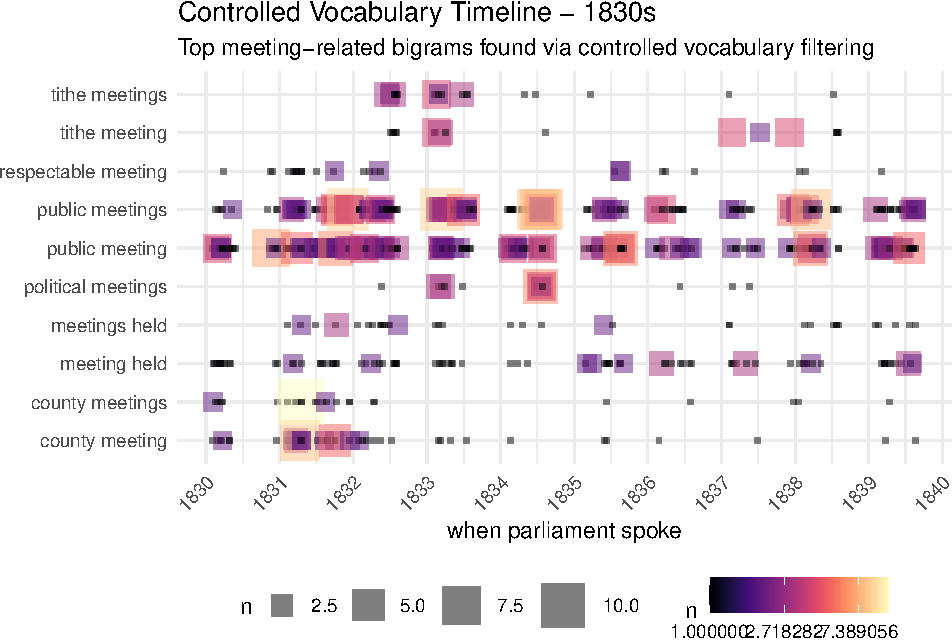
\includegraphics[keepaspectratio]{ch2_files/figure-latex/prob2_cv_1830s-1.pdf}}

\begin{Shaded}
\begin{Highlighting}[]
\FunctionTok{data}\NormalTok{(}\StringTok{"events"}\NormalTok{)}
\NormalTok{eventlist }\OtherTok{\textless{}{-}}\NormalTok{ events }\SpecialCharTok{\%\textgreater{}\%}
  \FunctionTok{distinct}\NormalTok{(event\_name, scholar\_assigned\_date) }\SpecialCharTok{\%\textgreater{}\%}
  \FunctionTok{filter}\NormalTok{(scholar\_assigned\_date }\SpecialCharTok{\textless{}=} \DecValTok{1840}\NormalTok{) }\SpecialCharTok{\%\textgreater{}\%}
  \FunctionTok{mutate}\NormalTok{(}\AttributeTok{event\_name =} \FunctionTok{str\_to\_lower}\NormalTok{(event\_name)) }\SpecialCharTok{\%\textgreater{}\%}
  \FunctionTok{select}\NormalTok{(event\_name, scholar\_assigned\_date)}

\FunctionTok{data}\NormalTok{(}\StringTok{"hansard\_1860"}\NormalTok{)}
\FunctionTok{data}\NormalTok{(}\StringTok{"debate\_metadata\_1860"}\NormalTok{)}

\NormalTok{h1860 }\OtherTok{\textless{}{-}} \FunctionTok{left\_join}\NormalTok{(hansard\_1860, debate\_metadata\_1860, }\AttributeTok{by =} \StringTok{"sentence\_id"}\NormalTok{) }\SpecialCharTok{\%\textgreater{}\%}
  \FunctionTok{mutate}\NormalTok{(}\AttributeTok{year =} \FunctionTok{year}\NormalTok{(speechdate),}
         \AttributeTok{text =} \FunctionTok{str\_to\_lower}\NormalTok{(text)) }\SpecialCharTok{\%\textgreater{}\%}
  \FunctionTok{filter}\NormalTok{(year }\SpecialCharTok{\textgreater{}=} \DecValTok{1860}\NormalTok{, year }\SpecialCharTok{\textless{}=} \DecValTok{1869}\NormalTok{)}

\NormalTok{get\_events\_year }\OtherTok{\textless{}{-}} \ControlFlowTok{function}\NormalTok{(y)\{}
\NormalTok{  h\_y }\OtherTok{\textless{}{-}}\NormalTok{ h1860 }\SpecialCharTok{\%\textgreater{}\%} \FunctionTok{filter}\NormalTok{(year }\SpecialCharTok{==}\NormalTok{ y)}
\NormalTok{  h\_y }\SpecialCharTok{\%\textgreater{}\%}
    \FunctionTok{unnest\_tokens}\NormalTok{(ngram, text, }\AttributeTok{token =} \StringTok{"ngrams"}\NormalTok{, }\AttributeTok{n =} \DecValTok{2}\NormalTok{) }\SpecialCharTok{\%\textgreater{}\%}
    \FunctionTok{inner\_join}\NormalTok{(eventlist, }\AttributeTok{by =} \FunctionTok{c}\NormalTok{(}\StringTok{"ngram"} \OtherTok{=} \StringTok{"event\_name"}\NormalTok{)) }\SpecialCharTok{\%\textgreater{}\%}
    \FunctionTok{select}\NormalTok{(ngram, speechdate, scholar\_assigned\_date)}
\NormalTok{\}}

\NormalTok{events\_1860s }\OtherTok{\textless{}{-}} \FunctionTok{bind\_rows}\NormalTok{(}\FunctionTok{lapply}\NormalTok{(}\DecValTok{1860}\SpecialCharTok{:}\DecValTok{1869}\NormalTok{, get\_events\_year))}

\NormalTok{counted }\OtherTok{\textless{}{-}}\NormalTok{ events\_1860s }\SpecialCharTok{\%\textgreater{}\%}
  \FunctionTok{mutate}\NormalTok{(}\AttributeTok{year =} \FunctionTok{year}\NormalTok{(speechdate)) }\SpecialCharTok{\%\textgreater{}\%}
  \FunctionTok{group\_by}\NormalTok{(ngram, year, speechdate, scholar\_assigned\_date) }\SpecialCharTok{\%\textgreater{}\%}
  \FunctionTok{summarize}\NormalTok{(}\AttributeTok{n =} \FunctionTok{n}\NormalTok{(), }\AttributeTok{.groups =} \StringTok{"drop"}\NormalTok{)}

\NormalTok{cleaned }\OtherTok{\textless{}{-}}\NormalTok{ counted }\SpecialCharTok{\%\textgreater{}\%}
  \FunctionTok{group\_by}\NormalTok{(ngram, scholar\_assigned\_date) }\SpecialCharTok{\%\textgreater{}\%}
  \FunctionTok{summarize}\NormalTok{(}\AttributeTok{total =} \FunctionTok{sum}\NormalTok{(n), }\AttributeTok{.groups =} \StringTok{"drop"}\NormalTok{) }\SpecialCharTok{\%\textgreater{}\%}
  \FunctionTok{arrange}\NormalTok{(scholar\_assigned\_date)}

\NormalTok{indexed }\OtherTok{\textless{}{-}}\NormalTok{ cleaned }\SpecialCharTok{\%\textgreater{}\%}
  \FunctionTok{mutate}\NormalTok{(}\AttributeTok{index =}\NormalTok{ scholar\_assigned\_date }\SpecialCharTok{\%/\%}\NormalTok{ ((}\FunctionTok{max}\NormalTok{(scholar\_assigned\_date) }\SpecialCharTok{{-}} \FunctionTok{min}\NormalTok{(scholar\_assigned\_date)) }\SpecialCharTok{/} \DecValTok{30}\NormalTok{)) }\SpecialCharTok{\%\textgreater{}\%}
  \FunctionTok{group\_by}\NormalTok{(index) }\SpecialCharTok{\%\textgreater{}\%}
  \FunctionTok{filter}\NormalTok{(total }\SpecialCharTok{==} \FunctionTok{max}\NormalTok{(total)) }\SpecialCharTok{\%\textgreater{}\%}
  \FunctionTok{ungroup}\NormalTok{() }\SpecialCharTok{\%\textgreater{}\%}
  \FunctionTok{left\_join}\NormalTok{(counted, }\AttributeTok{by =} \FunctionTok{c}\NormalTok{(}\StringTok{"ngram"}\NormalTok{, }\StringTok{"scholar\_assigned\_date"}\NormalTok{))}

\NormalTok{left\_range }\OtherTok{\textless{}{-}} \FunctionTok{max}\NormalTok{(events\_1860s}\SpecialCharTok{$}\NormalTok{speechdate) }\SpecialCharTok{+} \DecValTok{8}

\FunctionTok{ggplot}\NormalTok{(indexed, }\FunctionTok{aes}\NormalTok{(}\AttributeTok{x =}\NormalTok{ speechdate, }\AttributeTok{y =}\NormalTok{ scholar\_assigned\_date, }\AttributeTok{size =}\NormalTok{ n, }\AttributeTok{color =}\NormalTok{ n)) }\SpecialCharTok{+}
  \FunctionTok{geom\_point}\NormalTok{(}\AttributeTok{alpha =} \FloatTok{0.5}\NormalTok{, }\AttributeTok{shape =} \DecValTok{15}\NormalTok{) }\SpecialCharTok{+}
  \FunctionTok{scale\_color\_viridis}\NormalTok{(}\AttributeTok{trans =} \StringTok{"log"}\NormalTok{, }\AttributeTok{option =} \StringTok{"A"}\NormalTok{, }\AttributeTok{discrete =} \ConstantTok{FALSE}\NormalTok{) }\SpecialCharTok{+}
  \FunctionTok{scale\_size\_continuous}\NormalTok{(}\AttributeTok{range =} \FunctionTok{c}\NormalTok{(}\DecValTok{1}\NormalTok{, }\DecValTok{10}\NormalTok{)) }\SpecialCharTok{+}
  \FunctionTok{scale\_x\_date}\NormalTok{(}\AttributeTok{date\_breaks =} \StringTok{"1 year"}\NormalTok{, }\AttributeTok{date\_labels =} \StringTok{"\%Y"}\NormalTok{) }\SpecialCharTok{+}
  \FunctionTok{coord\_cartesian}\NormalTok{(}\AttributeTok{clip =} \StringTok{"off"}\NormalTok{) }\SpecialCharTok{+}
  \FunctionTok{geom\_text}\NormalTok{(}\AttributeTok{data =}\NormalTok{ indexed }\SpecialCharTok{\%\textgreater{}\%} \FunctionTok{group\_by}\NormalTok{(ngram) }\SpecialCharTok{\%\textgreater{}\%} \FunctionTok{sample\_n}\NormalTok{(}\DecValTok{1}\NormalTok{),}
            \FunctionTok{aes}\NormalTok{(}\AttributeTok{x =}\NormalTok{ left\_range, }\AttributeTok{y =}\NormalTok{ scholar\_assigned\_date,}
                \AttributeTok{label =} \FunctionTok{paste0}\NormalTok{(}\StringTok{"   "}\NormalTok{, ngram, }\StringTok{" ("}\NormalTok{, scholar\_assigned\_date, }\StringTok{")"}\NormalTok{)),}
            \AttributeTok{color =} \StringTok{"black"}\NormalTok{, }\AttributeTok{size =} \FloatTok{2.7}\NormalTok{, }\AttributeTok{hjust =} \DecValTok{0}\NormalTok{, }\AttributeTok{show.legend =} \ConstantTok{FALSE}\NormalTok{) }\SpecialCharTok{+}
  \FunctionTok{theme\_minimal}\NormalTok{() }\SpecialCharTok{+}
  \FunctionTok{theme}\NormalTok{(}\AttributeTok{axis.text.x =} \FunctionTok{element\_text}\NormalTok{(}\AttributeTok{angle =} \DecValTok{45}\NormalTok{, }\AttributeTok{hjust =} \DecValTok{1}\NormalTok{),}
        \AttributeTok{legend.position =} \StringTok{"bottom"}\NormalTok{,}
        \AttributeTok{plot.margin =} \FunctionTok{unit}\NormalTok{(}\FunctionTok{c}\NormalTok{(}\DecValTok{1}\NormalTok{, }\DecValTok{20}\NormalTok{, }\DecValTok{1}\NormalTok{, }\DecValTok{1}\NormalTok{), }\StringTok{"lines"}\NormalTok{)) }\SpecialCharTok{+}
  \FunctionTok{labs}\NormalTok{(}\AttributeTok{x =} \StringTok{"when parliament spoke"}\NormalTok{,}
       \AttributeTok{y =} \StringTok{"historical date of named event"}\NormalTok{,}
       \AttributeTok{title =} \StringTok{"Events Mentioned by Name {-} 1860s (eventlist)"}\NormalTok{,}
       \AttributeTok{subtitle =} \StringTok{"Earlier events (≤1840) referenced in 1860s debates"}\NormalTok{)}
\end{Highlighting}
\end{Shaded}

\pandocbounded{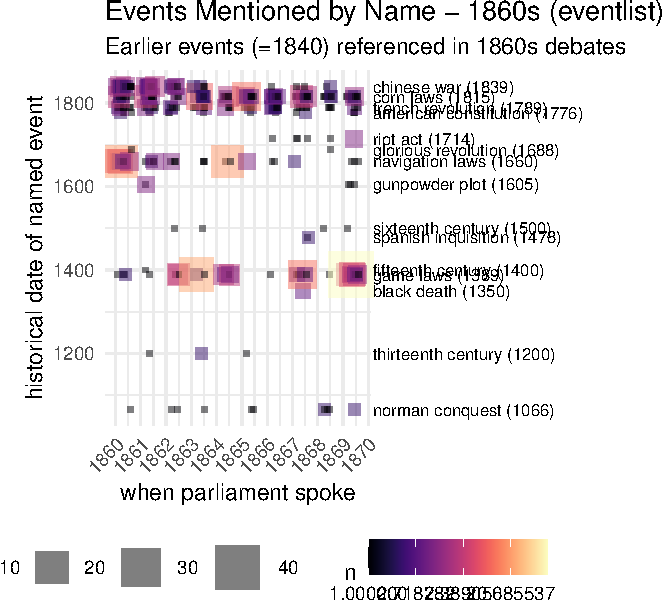
\includegraphics[keepaspectratio]{ch2_files/figure-latex/prob2_eventlist_1860s-1.pdf}}
which kinds of ``meeting'' phrases cluster in parliamentary speech
during the 1830s, and when do they spike?

\subsection{3) Analyze the results of your timelines. Use iterative
investigations of phrases, as modeled above, to conduct a distant
reading of the parliamentary speeches. Using at least ten examples,
compose a one-page essay investigating the question: how did
parliamentary speakers use references to contemporary and historical
events to make arguments for or against political
change?}\label{analyze-the-results-of-your-timelines.-use-iterative-investigations-of-phrases-as-modeled-above-to-conduct-a-distant-reading-of-the-parliamentary-speeches.-using-at-least-ten-examples-compose-a-one-page-essay-investigating-the-question-how-did-parliamentary-speakers-use-references-to-contemporary-and-historical-events-to-make-arguments-for-or-against-political-change}

\end{document}
